\chapter{Symbolic Heuristic Search}\label{ch:symbolic_heuristic_search}
\chapterquote{While the main observations of this paper are both intuitive and pretty obvious, I still consider the work a significant contribution in focusing attention on a key and often overlooked difference between explicit and symbolic search [\dots].}{Reviewer \#3 (2020)}

\section*{Core Publication of this Chapter}
\renewcommand{\citebf}[1]{\textbf{#1}}
\begin{itemize}
    \item \fullcite{speck-et-al-icaps2020}
\end{itemize}
\renewcommand{\citebf}[1]{#1}

Explicit search and symbolic search have been shown to be strong and competitive approaches for optimal classical planning.
While explicit search usually occurs as variants of forward \astar{} search \autocite{hart-et-al-ieeessc1968}, which are equipped with strong and efficient goal-distance heuristics, symbolic search is usually performed as (bidirectional) blind search, i.e., without heuristics.
This naturally raises the question of why not combine the two techniques to obtain a planning algorithm that combines the state pruning of explicit heuristic search with the concise representation of symbolic search.
This combination is referred to as symbolic heuristic search, which includes a variety of symbolic generalizations of \astar{} for different decision diagrams such as \bddastar{} \autocite{edelkamp-reffel-ki1998}, \addastar{} \autocite{hansen-et-al-sara2002} and \evmddastar{} \autocite{speck-et-al-icaps2018}.

The underlying idea of symbolic \astar{} search is to precompute and represent a \emph{heuristic function} $h$ with decision diagrams, where $h: \states \to \mathbb{N}_0 \cup \{ \infty \}$ such that $h(s_\star) = 0$ for all $s_\star \in \goalstates$.
Symbolic operations are then used to assign the corresponding $f$-values ($f = g + h$) to each state of a set of states $S_g$ reachable with cost $g$.
As usual with \astar{}, symbolic \astar{} expands the states in ascending order of the $f$-value and uses a tie-breaking rule in favor of states with smaller $g$-values \autocite{kissmann-edelkamp-aaai2011,torralba-phd2015}.
To guarantee optimal solutions, a \emph{consistent heuristic} is assumed, i.e., its estimate is always less than or equal to the estimated distance from each direct successor to the goal, plus the cost to reach that successor, i.e., $h(s) \leq h(s[o]) + \constcostfun(o)$.
Note that any consistent heuristic is also admissible, i.e., never overestimates the cost of reaching a goal state \autocite{pearl-1984}.
Two important examples of consistent heuristics and at the same time the extreme cases are the perfect heuristic $\perfecth{}$, which maps any state $s$ to the cost of the cheapest path from $s$ to any goal state, and the blind heuristic $\heu{blind}{}$, which maps any state $s$ to $0$.

\begin{figure}
    \centering
    \subfloat[First step.\label{fid:bddastar_example_a}]{
        \centering
        \makebox[0.5\textwidth][c]{
            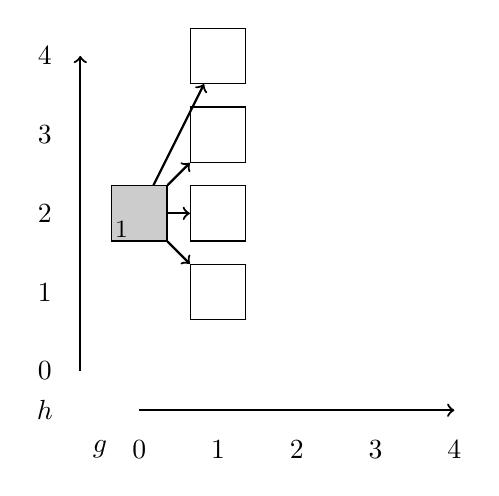
\begin{tikzpicture} [darkstyle/.style={draw,fill=gray!40,minimum size=20},scale=1]
    \path [draw, ->, thick] (0, -0.5) to (4, -0.5);
    \path [draw, ->, thick] (-0.75, 0) to (-0.75, 4);

    \node at (-0.5, -1) {$g$};
    \node at (-1.2, -0.5) {$h$};

    \foreach \x in {0,...,4}
    \node  at (1*\x,-1) {\x};

    \foreach \y in {0,...,4}
    \node  at (-1.2,1*\y) {\y};

    \foreach \x/\y/\i/\t in {0/2/1/ \init}{
            \node [darkstyle]  (\x\y) at (1*\x,1*\y) {\t};
            \node [] at (-0.225+\x, -0.2+\y)  {\small{$\i$}};
        }
    \foreach \x/\y in {1/1,1/2,1/3,1/4}{
            \node [draw, minimum size=20]  (\x\y) at (1*\x,1*\y) {};
        }
    \foreach \x/\y in {02/12, 02/11, 02/13, 02/14}{
            \path[draw, ->, thick] (\x) to (\y);
        }

\end{tikzpicture}
        }
    }
    \subfloat[Last step.\label{fid:bddastar_example_b}]{
        \centering
        \makebox[0.5\textwidth][c]{
            \begin{tikzpicture} [darkstyle/.style={draw,fill=gray!40,minimum size=20},scale=1]
    \path [draw, ->, thick] (0, -0.5) to (4, -0.5);
    \path [draw, ->, thick] (-0.75, 0) to (-0.75, 4);

    \node at (-0.5, -1) {$g$};
    \node at (-1.2, -0.5) {$h$};

    \foreach \x in {0,...,4}
    \node  at (1*\x,-1) {\x};

    \foreach \y in {0,...,4}
    \node  at (-1.2,1*\y) {\y};

    \foreach \x/\y/\i/\t in {0/2/1/ \init}{
            \node [darkstyle]  (\x\y) at (1*\x,1*\y) {\t};
            \node [] at (-0.225+\x, -0.2+\y)  {\small{$\i$}};
        }

    \foreach \x/\y/\i/\t in {1/1/2/, 1/2/3/, 2/1/4/, 1/3/5/, 2/2/6/, 3/1/7/,4/0/8/\goal}{
            \node [darkstyle]  (\x\y) at (1*\x,1*\y) {\t};
            \node [] at (-0.225+\x, -0.2+\y)  {\small{$\i$}};
        }

    \foreach \x/\y in {1/4,2/3,2/4,3/3,3/4,4/1,1/4,3/2}{
            \node [draw, minimum size=20]  (\x\y) at (1*\x,1*\y) {};
        }

    \foreach \x/\y in {02/12, 02/11, 02/13, 02/14, 11/21, 11/22, 12/21, 12/22, 12/23, 13/23,13/22,13/24,21/31,22/31,22/32,22/33,22/34,31/40,31/41}{
            \path[draw, ->, thick] (\x) to (\y);
        }


    \draw[dashed] (-0.0, 3.0) node [above] {\footnotesize $f=3$} -- (3.0, -0.0) ;
    \draw[dashed] (-0.0, 4.0) node [above] {\footnotesize $f=4$} -- (4.0, -0.0) ;

    \foreach \x/\y in {1/4,2/3,2/4,3/3,3/4,4/1,1/4,3/2}{
            \node [draw=red, sloped, cross out, line width=.5ex, minimum width=1.5ex, minimum height=1ex, anchor=center]  (\x\y) at (1*\x,1*\y) {};
        }

\end{tikzpicture}
        }
    }
    \caption[Illustration of BDDA$^\star$.]{Illustration of BDDA$^\star$, where the cells represent state sets $S_{g,h}$ and the arrows denote successor state sets. The gray cells are expanded in the order indicated by the numbers \autocite{torralba-gnad-icaps2017tutorial,torralba-phd2015}.
        %Inspired by similar visualizations of \textcite{torralba-phd2015,edelkamp-reffel-ki1998}.
    }
    \label{fid:bddastar_example}
\end{figure}

In \bddastar{}, a consistent heuristic function is precomputed and represented by multiple BDDs, one for each heuristic value $h$, where each BDD is used to represent the states $S_h$ with heuristic value $h$.
During search, states $S_g$ reachable with cost $g$ are partitioned according to their heuristic value by computing the intersections of $S_g$ and $S_h$ for each heuristic value $h$ resulting in sets of states $S_{g,h}$.
%
%As usual with \astar{}, \bddastar{} expands states in ascending order of $f = g + h$  and uses a tie-breaking rule in favor of states with smaller g-values \autocite{kissmann-edelkamp-aaai2011,torralba-phd2015}.
\Cref{ex:bddastar} exemplifies how \bddastar{} works.

\begin{example}\label{ex:bddastar}
    We consider a planning task with unit costs. \bddastar{} starts with the state set $S_{0,2} = \{ \init \}$, which contains only the initial state with a $g$-value of 0 and an $h$-value of $2$ (\Cref{fid:bddastar_example_a}).
    The expansion of $S_{0,2}$ leads to sets of states with $g$-value of $1$ and different $h$-values.
    Next, the state set $S_{1,1}$ is expanded, then $S_{1,2}$, and so on until a goal state is contained in $S_{4,0}$ (\Cref{fid:bddastar_example_b}).
\end{example}

While \bddastar{} utilizing a heuristic expands fewer states, symbolic blind search (\bddastar{} with $\heu{blind}{}$) potentially expands fewer sets of states.
Moreover, as \textcite{speck-et-al-icaps2020} have shown and we will examine in this chapter, the BDD representation of the state sets can deteriorate if the states are partitioned according to their $h$-values.
%In other words, in \bddastar{} the search fringe is described using symbolic representations and the notion of node expansions is generalized to region expansions as instead of single states represented as nodes whole sets of states are expanded.
%As all computations are performed with decision diagrams such that the concise presentation is maintained which then allows to expand the most promising states (minimal $f$-value) in form of a set of state represented as decision diagram.

There are several heuristics that can be precomputed and represented using symbolic search and decision diagrams, leading to cutting-edge performance in explicit heuristic search \autocite{edelkamp-aips2002,franco-et-al-ijcai2017,franco-et-al-ipc2018b,moraru-et-al-ki2019}.
Thus, all the ingredients are present to allow a symbolic planner utilizing heuristics, as explicit planners do.
However, \textcite{jensen-et-al-aij2008} identified the partitioning of state sets according to their heuristic values as a bottleneck, because multiple arithmetic operations have to be performed during search.
This leads to different extension of \bddastar{} to overcome this bottleneck such as Lazy \bddastar{} \autocite{torralba-phd2015}, which delays the heuristic evaluation as long as possible, or Set\astar{} \autocite{jensen-et-al-aij2008}, which encodes the heuristic values as preconditions of actions resulting in multiple actions with costs according to the heuristic values.
However, empirical evaluations show that all versions of \bddastar{} perform better than symbolic blind search in some domains but overall symbolic bidirectional search without any heuristic  performs best \autocite{torralba-et-al-ijcai2016}.

In the remainder of this chapter, we describe and summarize the results of \textcite{speck-et-al-icaps2020}, which theoretically and empirically evaluate the search behavior of \bddastar{}.
On the theoretical side, this study reveals another fundamental problem of symbolic heuristics, namely that the use of a heuristic does not always improve the search performance of \bddastar{}, as it may affect the size of the representation.
In general, even the \emph{perfect heuristic} can exponentially deteriorate the search performance of symbolic \astar{}.
The empirical evaluation is consistent with these theoretical results.
Finally, we conclude this chapter with a discussion of the implications of these
%theoretical and empirical results.
findings.

\begin{figure}
    \begin{center}
        %\resizebox{1\textwidth}{!}{
        \begin{tikzpicture}[%
		costnode/.style={pos=0.6,rectangle,thick,
				inner sep=2pt,draw,fill=white,text=black,font=\normalsize},%
		decisionnode/.style={circle,thick,minimum size=4mm,
				inner sep=2pt,draw,fill=white!80!black,text=black,font=\normalsize},%
		xscale=2,yscale=1.35,>=latex]
	\newcommand*{\lh}{0.6}%
	\newcommand*{\vh}{0.2}%

	\node[draw,thick,fill=white!80!black,rectangle, minimum size=0.55cm] (after0) at (1-7*\vh,0) {$0$};
	\node[decisionnode, minimum size=0.55cm] (x7) at (1-0*\vh,1*\lh) {$x_7$};
	\node[decisionnode, minimum size=0.55cm] (x6) at (1-1*\vh,2*\lh) {$x_6$};
	\node[decisionnode, minimum size=0.55cm] (x5) at (1-2*\vh,3*\lh) {$x_5$};
	\node[decisionnode, minimum size=0.55cm] (x4) at (1-3*\vh,4*\lh) {$x_4$};
	\node[decisionnode, minimum size=0.55cm] (x3) at (1-4*\vh,5*\lh) {$x_3$};
	\node[decisionnode, minimum size=0.55cm] (x2) at (1-5*\vh,6*\lh) {$x_2$};
	\node[decisionnode, minimum size=0.55cm] (x1) at (1-6*\vh,7*\lh) {$x_1$};
	\node[decisionnode, minimum size=0.55cm] (x0) at (1-7*\vh,8*\lh) {$x_0$};

	\node[] (tmp) at (1.1,2.3*\lh) {};

	\draw[->, thick] (1-7*\vh,9*\lh) -- (x0);

	\draw[->, thick,dotted] (x6.west) -- (after0);
	\draw[->, thick,dotted] (x5.west) -- (after0);
	\draw[->, thick,dotted] (x4.west) -- (after0);
	\draw[->, thick,dotted] (x3.west) -- (after0);
	\draw[->, thick,dotted] (x2.west) -- (after0);
	\draw[->, thick,dotted] (x1.west) -- (after0);
	\draw[->, thick,dotted] (x0.west) -- (after0);

	\draw[->, thick] (x7) -- (after0);
	\draw[->, thick] (x6.east) to[bend left=10] (x7);
	\draw[->, thick] (x5.east) to[bend left=10] (x6);
	\draw[->, thick] (x4.east) to[bend left=10] (x5);
	\draw[->, thick] (x3.east) to[bend left=10] (x4);
	\draw[->, thick] (x2.east) to[bend left=10] (x3);
	\draw[->, thick] (x1.east) to[bend left=10] (x2);
	\draw[->, thick] (x0.east) to[bend left=10] (x1);

	%%%%%%%%% Additional 1 node
	\renewcommand{\vh}{2.4}

	\node[draw,thick,fill=white!80!black,rectangle, minimum size=0.55cm] (blind) at (\vh,0*\lh) {$1$};


	%%%%%%%%% Exponential BDD

	\renewcommand*{\lh}{0.8}%
	\renewcommand{\vh}{4.2}

	\node[draw,thick,fill=white!80!black,rectangle, minimum size=0.55cm] (after0) at (\vh-0.5,0*\lh) {$0$};
	\node[draw,thick,fill=white!80!black,rectangle, minimum size=0.55cm] (after1) at (\vh+0.5,0*\lh) {$1$};

	\node[decisionnode, minimum size=0.55cm] (v6) at (\vh-0.25,1*\lh) {$v_6$};

	\node[decisionnode, minimum size=0.55cm] (v50) at (\vh-0.25,2*\lh) {$v_5$};
	\node[decisionnode, minimum size=0.55cm] (v51) at (\vh+0.25,2*\lh) {$v_5$};

	\node[decisionnode, minimum size=0.55cm] (v40) at (\vh-0.25,3*\lh) {$v_4$};
	\node[decisionnode, minimum size=0.55cm] (v41) at (\vh+0.25,3*\lh) {$v_4$};
	\node[decisionnode, minimum size=0.55cm] (v42) at (\vh+0.75,3*\lh) {$v_4$};
	\node[decisionnode, minimum size=0.55cm] (v43) at (\vh+1.25,3*\lh) {$v_4$};

	\node[decisionnode, minimum size=0.55cm] (v30) at (\vh+-1.25,4*\lh) {$v_3$};
	\node[decisionnode, minimum size=0.55cm] (v31) at (\vh+-0.75,4*\lh) {$v_3$};
	\node[decisionnode, minimum size=0.55cm] (v32) at (\vh+-0.25,4*\lh) {$v_3$};
	\node[decisionnode, minimum size=0.55cm] (v33) at (\vh+0.25,4*\lh) {$v_3$};

	\node[decisionnode, minimum size=0.55cm] (v20) at (\vh+-1,5*\lh) {$v_2$};
	\node[decisionnode, minimum size=0.55cm] (v21) at (\vh+0,5*\lh) {$v_2$};

	\node[decisionnode, minimum size=0.55cm] (v1) at (\vh+-0.5,6*\lh) {$v_1$};

	\draw[->, thick,dotted] (v6) -- (after0);
	\draw[->, thick] (v6) -- (after1);

	\draw[->, thick,dotted] (v50) to[bend right=10]  (after0);
	\draw[->, thick] (v50) -- (after1);

	\draw[->, thick,dotted] (v51) -- (v6);
	\draw[->, thick] (v51) -- (after1);

	\draw[->, thick,dotted] (v40) to[bend right=15] (after0);
	\draw[->, thick] (v40) -- (after1);

	\draw[->, thick,dotted] (v41) -- (v6);
	\draw[->, thick] (v41) to[bend left=10]  (after1);

	\draw[->, thick,dotted] (v42) -- (v50);
	\draw[->, thick] (v42) -- (after1);

	\draw[->, thick,dotted] (v43) -- (v51);
	\draw[->, thick] (v43) -- (after1);

	\draw[->, thick,dotted] (v30) -- (after0);
	\draw[->, thick] (v30) -- (v6);

	\draw[->, thick,dotted] (v31) -- (v50);
	\draw[->, thick] (v31) to[bend left=24] (v51);

	\draw[->, thick,dotted] (v32) -- (v40);
	\draw[->, thick] (v32) -- (v41);

	\draw[->, thick,dotted] (v33) -- (v42);
	\draw[->, thick] (v33) -- (v43);

	\draw[->, thick,dotted] (v20) -- (v30);
	\draw[->, thick] (v20) -- (v31);

	\draw[->, thick,dotted] (v21) -- (v32);
	\draw[->, thick] (v21) -- (v33);

	\draw[->, thick,dotted] (v1) -- (v20);
	\draw[->, thick] (v1) -- (v21);


	%%%%%%% Inter drawing
	\draw[->,thick,dotted] (x7.east) |- node[costnode, pos=0.75] {with $\perfecth$} (v1);

	\draw[->,thick,dotted] (tmp) -| node[costnode, pos=0.25] {with $\heu{blind}{}$} (blind.north);
	%(blind.north)

	%\node[] at (-1.5,6*\lh) {B:};
	%\node[draw,thick,fill=white!80!black,regular polygon,regular polygon sides=3, minimum size=0.55cm] (B) at (0.25,6.5*\lh) {B};
	%\draw[->, thick,dotted] (-0.0,6.25*\lh) -- (a1);
\end{tikzpicture}
        %}
    \end{center}
    \caption[Visualization of two BDDs with exponential size difference.]{
        Visualization of two BDDs $B_S$ (with $h_{\text{\scriptsize blind}}$) and $B_{S'}$ (with $h_{\scriptsize \star}$) representing state sets $S$ and $S'$, where $B_{S'}$ is exponentially larger in the number of variables than $B_{S}$, although $S' \subsetneq S$ \autocite{speck-et-al-icaps2020}.}
    \label{fid:bddastar_proof}
\end{figure}

\section{Theoretical Results}

\textcite{speck-et-al-icaps2020} show that good goal-distance estimations in the form of heuristics are not the appropriate quantity to improve the search performance of symbolic heuristic search.
The reason for this is that, in contrast to explicit \astar{}, where every
consistent heuristic can only reduce the number of necessary node expansions (up to tie-breaking) and thus the search effort compared to blind search, in \bddastar{} no such guarantee exists.
In \bddastar{}, the size of expanded BDDs, i.e., number of BDD nodes, representing expanded states determines the search effort and thus the runtime.
As a BDD $B_{S'}$ can be exponentially larger than a BDD $B_{S}$ although the set of states $S'$ is a strict subset of $S$, i.e., $S' \subsetneq S$, it is not always beneficial to represent and expand fewer states (\Cref{fid:bddastar_proof}).
In other words, in explicit search, where the most promising states (search fringe) are simply enumerated explicitly, reducing the number of states to expand directly improves search performance.
However, in symbolic search, reducing the number of states to be expanded can lead to a larger representation size in form of BDDs and a fragmentation of the search fringe as the search progresses.

Similar to \say{must-expand} nodes in explicit search, \textcite{speck-et-al-icaps2020} introduce the notion of \emph{expansion size} for \bddastar{} as the cumulative size of BDDs that must always be expanded by \bddastar{} before finding an optimal solution to measure search effort.
Using this notion it is possible to prove that even under the best possible and unrealistic circumstances, namely the perfect heuristic, the search effort of \bddastar{} can be exponentially larger than the search effort of symbolic
search without heuristic, and vice versa (\Cref{thm:bddastar}).

\begin{theorem}[\cite{speck-et-al-icaps2020}]\label{thm:bddastar}
    Using the perfect heuristic $\perfecth$ instead of the blind heuristic $\heu{blind}{}$ can \emph{decrease} or \emph{increase} the expansion size of \bddastar{} exponentially in the size of the planning task for a given variable ordering. \qed
\end{theorem}

While the result that the search performance of \bddastar{} can be exponentially improved when $\perfecth$ is used instead of $\heu{blind}{}$ is less surprising, the opposite result is very surprising.
This highlights the difference between explicit and symbolic search: the representation of the search fringe must be concise, and in symbolic search the decision diagram size is not directly related to the number of states represented.
To prove that using $\perfecth$ instead of $\heu{blind}{}$ can exponentially increase the expansion size and thus exponentially deteriorate search performance, \textcite{speck-et-al-icaps2020} constructed a family of planning tasks $\task_n$ parameterized over the number of (relevant) variables.
Solving tasks of this family of planning tasks $\task_n$ with \bddastar{} using the perfect heuristic prunes states from the expanded set of states (search fringe) so that the representation size increases exponentially.
\Cref{fid:bddastar_proof} shows the core idea of the proof, with two BDDs representing the search fringe, i.e., the expanded state set, in the last expansion step of \bddastar{} using $\perfecth$ or $\heu{blind}{}$ when solving $\task_3$.
The key observation is that when $\heu{blind}{}$ is used, no states are pruned according to their values over variables $v_i$, resulting in a compact BDD representation.
However, if $\perfecth$ is used, states are pruned according to their values over the variables $v_i$ and the function $(v_1 \land v_{n+1}) \lor \dots \lor (v_{n} \land v_{2n})$ has to be represented, which under certain variable orders requires a BDD with exponentially many nodes \autocite{kissmann-phd2012}.

Finally, \textcite{speck-et-al-icaps2020} show that these theoretical results also hold for several other symbolic \astar{} variants such as Lazy \bddastar{}, Set\astar{}, \addastar{}, and \evmddastar{}, as well as for their bidirectional extensions.

\begin{figure}
    \subfloat[Search Effort (BDD nodes)\label{fig:bddastar_data_a}]{
        \centering
        \makebox[1\textwidth][c]{
            \resizebox{0.95\textwidth}{!}{
                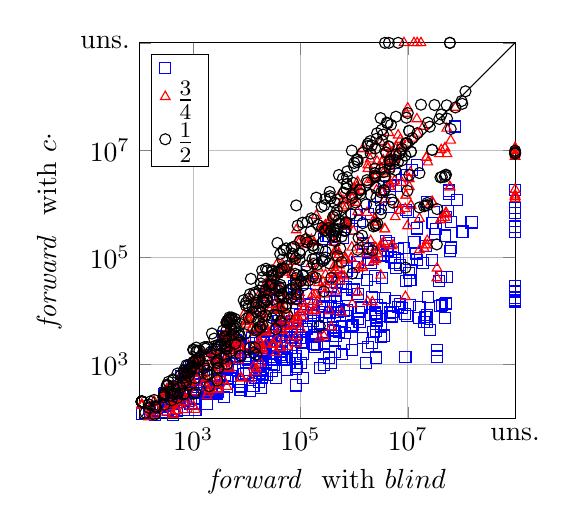
\begin{tikzpicture}[scale=1]
\begin{axis}[grid=major,height=2.5in, legend cell align=right, width=2.5in,xlabel style={align=center}, xlabel={\emph{forward} \bddastar{} with $\heu{blind}{}$}, xmin=100, xmax=1000000001, xmode=log, ylabel style={align=center}, ylabel={\emph{forward} \bddastar{} with $c \cdot \perfecth$}, ymin=100, ymax=1000000001, ymode=log,legend pos=north west, xticklabels={$10^3$, $10^5$, $10^7$, uns.},yticklabels={$10^3$, $10^5$, $10^7$, uns.}]
%legend style={anchor=north east}
\addplot[only marks,mark=square,blue] coordinates {
(1000000000, 302844.000000) (1000000000, 1827870.000000) (1000000000, 302844.000000)
(45711.000000, 1202.000000) (2522080.000000, 1359.000000) (2455.000000, 1743.000000) (4658.000000, 2753.000000) (9126.000000, 1346.000000) (523593.000000, 11024.000000) (4204700.000000, 134957.000000) (2903.000000, 320.000000) (1063080.000000, 610142.000000) (3472030.000000, 108515.000000) (22153400.000000, 162822.000000) (22250.000000, 20175.000000) (132902.000000, 52438.000000) (58676300.000000, 1512240.000000) (10571800.000000, 93101.000000) (6213.000000, 2824.000000) (55378.000000, 2005.000000) (23113700.000000, 6225.000000) (418.000000, 117.000000) (79252.000000, 1286.000000) (111298.000000, 572.000000) (7054320.000000, 13356.000000) (2602800.000000, 7598.000000) (41995.000000, 2799.000000) (44613.000000, 1707.000000) (2615370.000000, 12857.000000) (5886.000000, 1630.000000) (276895.000000, 11893.000000) (2554.000000, 1534.000000) (501.000000, 137.000000) (54262.000000, 5680.000000) (1291640.000000, 475132.000000) (1000000000, 15496.000000) (27975400.000000, 437052.000000) (4063040.000000, 163801.000000) (9401240.000000, 761732.000000) (2635.000000, 364.000000) (972.000000, 350.000000) (3935890.000000, 199703.000000) (730606.000000, 19582.000000) (733209.000000, 10557.000000) (32991.000000, 2637.000000) (1022.000000, 511.000000) (337.000000, 144.000000) (4394280.000000, 873920.000000) (16874.000000, 7152.000000) (4632.000000, 2751.000000) (681.000000, 657.000000) (101586.000000, 2642.000000) (995.000000, 540.000000) (3295500.000000, 41207.000000) (110.000000, 119.000000) (4.000000, 4.000000) (8970200.000000, 8798.000000) (6019750.000000, 62347.000000) (5106.000000, 2374.000000) (3731820.000000, 17785.000000) (49299600.000000, 255355.000000) (730606.000000, 19582.000000) (41816.000000, 5166.000000) (2431710.000000, 9384.000000) (374063.000000, 1093.000000) (83169.000000, 844.000000) (5307690.000000, 9571.000000) (1000000000, 22539.000000) (75380.000000, 17464.000000) (66949.000000, 2064.000000) (681322.000000, 3883.000000) (5854060.000000, 96221.000000) (5810980.000000, 15177.000000) (10.000000, 10.000000) (110.000000, 119.000000) (10803.000000, 797.000000) (110.000000, 119.000000) (3935890.000000, 199703.000000) (110.000000, 119.000000) (110.000000, 119.000000) (252402.000000, 96632.000000) (34759900.000000, 1865.000000) (4109.000000, 3301.000000) (5216.000000, 1745.000000) (622431.000000, 233109.000000) (53769700.000000, 43684.000000) (48843300.000000, 7529.000000) (3136420.000000, 3335.000000) (296101.000000, 7857.000000) (453599.000000, 3409.000000) (3559180.000000, 3495.000000) (9193550.000000, 36635.000000) (6125.000000, 2888.000000) (16460600.000000, 7401.000000) (7759860.000000, 11386.000000) (110.000000, 119.000000) (1324960.000000, 11662.000000) (22349.000000, 1057.000000) (20152700.000000, 6200.000000) (42815.000000, 1373.000000) (1000000000, 14487.000000) (55426.000000, 1300.000000) (878445.000000, 5099.000000) (70.000000, 81.000000) (292.000000, 130.000000) (104647000.000000, 303555.000000) (15754.000000, 921.000000) (29533.000000, 1020.000000) (62876700.000000, 453888.000000) (110.000000, 119.000000) (378.000000, 277.000000) (11863.000000, 1989.000000) (11393.000000, 1459.000000) (14942100.000000, 347116.000000) (14918.000000, 568.000000) (583095.000000, 5134.000000) (16.000000, 16.000000) (2523140.000000, 5789.000000) (82394.000000, 31788.000000) (1305.000000, 697.000000) (206094.000000, 2339.000000) (2393440.000000, 872487.000000) (3973.000000, 2191.000000) (820.000000, 506.000000) (13302600.000000, 196412.000000) (507.000000, 305.000000) (404711.000000, 152731.000000) (2175890.000000, 2516.000000) (5036.000000, 621.000000) (50937100.000000, 576224.000000) (671.000000, 572.000000) (10702.000000, 1218.000000) (5227.000000, 916.000000) (287.000000, 266.000000) (30302.000000, 1279.000000) (288.000000, 288.000000) (2514210.000000, 4206.000000) (29881.000000, 763.000000) (97162.000000, 7324.000000) (733.000000, 226.000000) (1000000000, 17353.000000) (9568.000000, 1084.000000) (692176.000000, 8073.000000) (41641.000000, 4310.000000) (110.000000, 119.000000) (11429000.000000, 59046.000000) (3731820.000000, 17785.000000) (76890600.000000, 27554800.000000) (1106.000000, 1078.000000) (53126500.000000, 43854.000000) (110.000000, 119.000000) (4656960.000000, 1671150.000000) (344692.000000, 1358.000000) (11429000.000000, 59046.000000) (418.000000, 117.000000) (58867400.000000, 1765140.000000) (29893900.000000, 438675.000000) (3819.000000, 3323.000000) (1319.000000, 477.000000) (1000000000, 681384.000000) (19997.000000, 1832.000000) (4713.000000, 1271.000000) (35723.000000, 2127.000000) (14169.000000, 562.000000) (18016.000000, 366.000000) (1589.000000, 380.000000) (3845.000000, 2476.000000) (2442920.000000, 8661.000000) (133168.000000, 13591.000000) (3271240.000000, 41151.000000) (3344.000000, 1517.000000) (644193.000000, 10086.000000) (445022.000000, 4189.000000) (1983260.000000, 123704.000000) (2740.000000, 515.000000) (1691.000000, 1323.000000) (41339.000000, 1520.000000) (696.000000, 362.000000) (13553.000000, 2043.000000) (45890.000000, 1809.000000) (19365.000000, 566.000000) (7039.000000, 2291.000000) (22153400.000000, 162822.000000) (4969510.000000, 7920.000000) (394.000000, 196.000000) (16.000000, 24.000000) (8487580.000000, 147719.000000) (1157410.000000, 7229.000000) (14143.000000, 2095.000000) (365081.000000, 28053.000000) (90.000000, 88.000000) (5689.000000, 1423.000000) (41129.000000, 26546.000000) (407682.000000, 4930.000000) (38913.000000, 6480.000000) (271848.000000, 1004.000000) (31260900.000000, 708601.000000) (19674.000000, 672.000000) (1157090.000000, 82873.000000) (478.000000, 202.000000) (4308.000000, 954.000000) (10.000000, 10.000000) (74.000000, 82.000000) (1000000000, 29804.000000) (1783250.000000, 2120.000000) (617650.000000, 33580.000000) (802.000000, 211.000000) (276.000000, 166.000000) (169910.000000, 6457.000000) (110.000000, 119.000000) (5963.000000, 862.000000) (33156700.000000, 337428.000000) (82022.000000, 1086.000000) (4333.000000, 898.000000) (365988.000000, 12593.000000) (1674760.000000, 1059.000000) (523593.000000, 11024.000000) (110.000000, 119.000000) (573.000000, 241.000000) (48193.000000, 5024.000000) (279415.000000, 220677.000000) (918553.000000, 340794.000000) (70566.000000, 6528.000000) (68120.000000, 3310.000000) (110.000000, 119.000000) (2703870.000000, 6471.000000) (1205250.000000, 9429.000000) (169910.000000, 6457.000000) (154216000.000000, 448997.000000) (4564760.000000, 2121140.000000) (1005910.000000, 25218.000000) (10970400.000000, 12838.000000) (1731790.000000, 37821.000000) (744.000000, 690.000000) (2442920.000000, 8661.000000) (30.000000, 30.000000) (2124420.000000, 17976.000000) (4223.000000, 536.000000) (1141.000000, 587.000000) (1161.000000, 427.000000) (159507.000000, 12773.000000) (25640100.000000, 4367.000000) (439967.000000, 14533.000000) (16464600.000000, 11774.000000) (174830.000000, 8378.000000) (157.000000, 131.000000) (517387.000000, 4122.000000) (639.000000, 319.000000) (110.000000, 119.000000) (4658.000000, 2753.000000) (1896.000000, 281.000000) (961702.000000, 5562.000000) (4241.000000, 388.000000) (110.000000, 119.000000) (292.000000, 288.000000) (10571800.000000, 93101.000000) (2485270.000000, 27775.000000) (178023.000000, 10371.000000) (205.000000, 154.000000) (31872.000000, 999.000000) (196995.000000, 31408.000000) (4613830.000000, 9437.000000) (1113000.000000, 51699.000000) (1139.000000, 570.000000) (793.000000, 479.000000) (97162.000000, 7324.000000) (44506.000000, 2187.000000) (13.000000, 20.000000) (37080.000000, 12962.000000) (110.000000, 119.000000) (909.000000, 326.000000) (110.000000, 119.000000) (1000000000, 16158.000000) (111298.000000, 572.000000) (349608.000000, 9224.000000) (290015.000000, 9630.000000) (7782.000000, 393.000000) (27653.000000, 3562.000000) (299457.000000, 247181.000000) (4434830.000000, 183911.000000) (1088.000000, 243.000000) (154216000.000000, 448997.000000) (19263.000000, 2086.000000) (49577.000000, 1371.000000) (191.000000, 117.000000) (878445.000000, 5099.000000) (27873.000000, 24671.000000) (56136.000000, 3584.000000) (519863.000000, 40343.000000) (14987.000000, 2037.000000) (167152.000000, 3224.000000) (477734.000000, 12011.000000) (292.000000, 297.000000) (1402830.000000, 11623.000000) (3191990.000000, 1161890.000000) (581.000000, 626.000000) (22709.000000, 5355.000000) (1000000000, 681384.000000) (2771.000000, 289.000000) (1798.000000, 304.000000) (2864.000000, 312.000000) (10668800.000000, 51927.000000) (904088.000000, 5305.000000) (434344.000000, 15279.000000) (1000000000, 840227.000000) (75380.000000, 17464.000000) (254977.000000, 6082.000000) (149.000000, 147.000000) (80793.000000, 1454.000000) (287.000000, 266.000000) (23011800.000000, 8327.000000) (110.000000, 119.000000) (4215.000000, 576.000000) (7054320.000000, 13356.000000) (32326900.000000, 272010.000000) (2682.000000, 298.000000) (100141.000000, 1076.000000) (713553.000000, 423167.000000) (23649900.000000, 18511.000000) (113038.000000, 4136.000000) (677.000000, 218.000000) (2868.000000, 396.000000) (9021340.000000, 1381.000000) (263252.000000, 3497.000000) (110.000000, 119.000000) (274332.000000, 2485.000000) (110.000000, 119.000000) (109460.000000, 10746.000000) (40221.000000, 3238.000000) (22714.000000, 1099.000000) (7466.000000, 1712.000000) (584407.000000, 1604.000000) (434344.000000, 15279.000000) (83156300.000000, 1163280.000000) (4284.000000, 2743.000000) (1814.000000, 361.000000) (53231.000000, 1205.000000) (1154720.000000, 20470.000000) (83206.000000, 410.000000) (983.000000, 685.000000) (29101.000000, 26582.000000) (110.000000, 119.000000) (1000000000, 23490.000000) (710791.000000, 28467.000000) (2485270.000000, 27775.000000) (26.000000, 26.000000) (18127.000000, 829.000000) (35074800.000000, 1417.000000) (40610600.000000, 12242.000000) (12054.000000, 2533.000000) (48346.000000, 6358.000000) (174934.000000, 2461.000000) (1000000000, 14561.000000) (3745.000000, 248.000000) (1097.000000, 145.000000) (16.000000, 24.000000) (27.000000, 27.000000) (5656380.000000, 78806.000000) (28.000000, 33.000000) (19375.000000, 1915.000000) (2918.000000, 883.000000) (421.000000, 264.000000) (1838.000000, 368.000000) (2819.000000, 384.000000) (16.000000, 24.000000) (36.000000, 42.000000) (213230.000000, 8379.000000) (6978.000000, 481.000000) (12133700.000000, 4314210.000000) (97782.000000, 8535.000000) (920.000000, 920.000000) (11425.000000, 324.000000) (110.000000, 119.000000) (87368.000000, 906.000000) (1105.000000, 1078.000000) (74.000000, 61.000000) (5274.000000, 793.000000) (756.000000, 756.000000) (60870000.000000, 131199.000000) (5700140.000000, 3595260.000000) (901841.000000, 25222.000000) (4219.000000, 825.000000) (2288630.000000, 4056.000000) (187201.000000, 2116.000000) (12682.000000, 3209.000000) (7270600.000000, 71018.000000) (28415700.000000, 90537.000000) (17237.000000, 694.000000) (34623.000000, 568.000000) (2104.000000, 392.000000) (18136.000000, 1588.000000) (3190060.000000, 11309.000000) (16.000000, 16.000000) (418.000000, 117.000000) (90.000000, 88.000000) (714.000000, 291.000000) (6528680.000000, 11983.000000) (1311.000000, 412.000000) (50571800.000000, 13618.000000) (1000000000, 375711.000000) (491188.000000, 9675.000000) (3165540.000000, 5002.000000) (15073.000000, 1518.000000) (70566.000000, 6528.000000) (67531.000000, 4157.000000) (19486000.000000, 77994.000000) (2226.000000, 315.000000) (1011.000000, 189.000000) (20064.000000, 2534.000000) (110.000000, 119.000000) (14743.000000, 3363.000000) (9544.000000, 702.000000) (39654.000000, 4687.000000) (110.000000, 119.000000) (8719.000000, 673.000000) (2027800.000000, 8336.000000) (3973.000000, 2191.000000) (56166100.000000, 725079.000000) (110.000000, 119.000000) (4613830.000000, 7864.000000) (72.000000, 59.000000) (95988.000000, 3096.000000) (2676130.000000, 112459.000000) (15069100.000000, 5341000.000000) (13009700.000000, 440511.000000) (1571.000000, 585.000000) (4136.000000, 985.000000) (56553.000000, 789.000000) (16.000000, 24.000000) (7718180.000000, 2750960.000000) (10.000000, 10.000000) (11192900.000000, 37769.000000) (24105.000000, 2700.000000) (110.000000, 119.000000) (228149.000000, 877.000000) (29210.000000, 2341.000000) (1798160.000000, 88951.000000) (128.000000, 62.000000) (9193550.000000, 36635.000000) (1790630.000000, 654921.000000) (923044.000000, 1855.000000) (439967.000000, 14533.000000) (26332.000000, 24996.000000) (6072.000000, 787.000000) (6604110.000000, 142208.000000) (96.000000, 104.000000) (1799.000000, 185.000000) (919.000000, 343.000000) (60870000.000000, 131199.000000) (37261.000000, 15531.000000) (29793.000000, 3130.000000) (3108960.000000, 108044.000000) (63038600.000000, 152491.000000) (1628.000000, 1517.000000) (74398.000000, 29393.000000) (519.000000, 205.000000) (14300600.000000, 118317.000000) (43150000.000000, 12842.000000) (88474.000000, 18879.000000) (1969.000000, 323.000000) (186.000000, 140.000000) (110.000000, 119.000000) (1447210.000000, 3126.000000) (4297.000000, 2320.000000) (6016530.000000, 2152650.000000) (4394280.000000, 873920.000000) (4779.000000, 551.000000) (128700.000000, 4653.000000) (346.000000, 174.000000) (483800.000000, 34069.000000) (214539.000000, 5030.000000) (445894.000000, 1755.000000) (41932600.000000, 42698.000000) (22559200.000000, 1075780.000000) (890.000000, 187.000000) (991506.000000, 66159.000000) (148.000000, 90.000000) (59.000000, 66.000000) (3192.000000, 679.000000) (7592.000000, 338.000000) (109385.000000, 1559.000000) (33.000000, 36.000000) (19723.000000, 1824.000000) (354183.000000, 18181.000000) (383.000000, 189.000000) (17195.000000, 966.000000) (4142.000000, 943.000000) (48467.000000, 4346.000000) (319.000000, 176.000000) (2933.000000, 345.000000) (44282.000000, 2605.000000) (418.000000, 117.000000) (7507.000000, 2078.000000) (5087.000000, 2738.000000) (1788920.000000, 151121.000000) (1012.000000, 793.000000) (1446720.000000, 181708.000000) (51380400.000000, 14138.000000) (110.000000, 119.000000) (13255.000000, 396.000000) (20612.000000, 2691.000000) (710791.000000, 28467.000000) (80588.000000, 2936.000000) (196.000000, 163.000000) (21371600.000000, 7634.000000) (14751300.000000, 89003.000000) (1259510.000000, 6319.000000) (49299600.000000, 255355.000000) (87194.000000, 3576.000000) (3598.000000, 3456.000000) (65569.000000, 3115.000000) (154413.000000, 9335.000000) (4604750.000000, 9172.000000) (9824100.000000, 8223.000000) (110.000000, 119.000000) (2031610.000000, 78701.000000) (30715.000000, 1391.000000) (110.000000, 119.000000) (292470.000000, 18292.000000) (38626600.000000, 35809.000000) (110.000000, 119.000000) (190561.000000, 3544.000000) (170911.000000, 2433.000000) (1220.000000, 1171.000000) (422.000000, 276.000000) (10747.000000, 2488.000000) (246880.000000, 12492.000000) (741597.000000, 55254.000000) (661.000000, 144.000000) (3555040.000000, 2549870.000000) (21258.000000, 1687.000000) (4847020.000000, 101165.000000) (140940.000000, 5041.000000) (1273.000000, 1153.000000) (9750820.000000, 3479930.000000) (649749.000000, 2425.000000) (3956.000000, 631.000000) (18248.000000, 1447.000000) (83086.000000, 14259.000000) (549606.000000, 8106.000000) (54.000000, 54.000000) (332024.000000, 249266.000000) (73.000000, 70.000000) (9966760.000000, 696838.000000) (1156.000000, 345.000000) (28415700.000000, 90537.000000) (432.000000, 152.000000) (125800.000000, 20982.000000) (324.000000, 215.000000) (23960.000000, 642.000000) (16669.000000, 484.000000) (2451700.000000, 45432.000000) (407326.000000, 4398.000000)
};
\addlegendentry{\large$\perfecth$}

\addplot[only marks,mark=triangle,red] coordinates {
(1000000000, 11014400.000000) (1000000000, 11014400.000000)
(14942100.000000, 1000000000) (8487580.000000, 1000000000) (17590000.000000, 1000000000) (13009700.000000, 1000000000)
(681322.000000, 97687.000000) (45711.000000, 72965.000000) (2903.000000, 893.000000) (2522080.000000, 152144.000000) (2455.000000, 1878.000000) (4658.000000, 7222.000000) (9126.000000, 1640.000000) (523593.000000, 71648.000000) (4204700.000000, 11201500.000000) (1063080.000000, 1057000.000000) (3472030.000000, 6551310.000000) (22153400.000000, 7281280.000000) (22250.000000, 24638.000000) (132902.000000, 178928.000000) (10571800.000000, 2917820.000000) (6213.000000, 3127.000000) (55378.000000, 5149.000000) (23113700.000000, 169929.000000) (418.000000, 117.000000) (79252.000000, 15033.000000) (7054320.000000, 743441.000000) (2602800.000000, 131071.000000) (41995.000000, 10293.000000) (44613.000000, 10202.000000) (2615370.000000, 1792760.000000) (5886.000000, 2142.000000) (276895.000000, 373836.000000) (2554.000000, 1500.000000) (54262.000000, 60197.000000) (1291640.000000, 1767190.000000) (1000000000, 7599380.000000) (4063040.000000, 11605200.000000) (9401240.000000, 48211000.000000) (22153400.000000, 7281280.000000) (972.000000, 493.000000) (3935890.000000, 3612450.000000) (730606.000000, 416304.000000) (733209.000000, 905710.000000) (32991.000000, 10773.000000) (1022.000000, 1189.000000) (337.000000, 303.000000) (4394280.000000, 6934300.000000) (16874.000000, 19859.000000) (4632.000000, 7184.000000) (681.000000, 594.000000) (101586.000000, 9129.000000) (995.000000, 1235.000000) (3295500.000000, 1593670.000000) (110.000000, 176.000000) (4.000000, 4.000000) (8970200.000000, 805029.000000) (6019750.000000, 11731900.000000) (5106.000000, 5291.000000) (3731820.000000, 336918.000000) (49299600.000000, 10889600.000000) (730606.000000, 416304.000000) (41816.000000, 52877.000000) (2431710.000000, 452481.000000) (374063.000000, 5041.000000) (83169.000000, 3297.000000) (581.000000, 626.000000) (5307690.000000, 169018.000000) (1000000000, 9786620.000000) (75380.000000, 83957.000000) (66949.000000, 5452.000000) (60870000.000000, 2049950.000000) (681322.000000, 97687.000000) (5854060.000000, 10623700.000000) (5810980.000000, 568977.000000) (10.000000, 10.000000) (110.000000, 176.000000) (10803.000000, 2241.000000) (110.000000, 176.000000) (3935890.000000, 3612450.000000) (110.000000, 176.000000) (110.000000, 176.000000) (252402.000000, 341043.000000) (34759900.000000, 41419.000000) (4109.000000, 3301.000000) (5216.000000, 1787.000000) (622431.000000, 849351.000000) (53769700.000000, 8515530.000000) (48843300.000000, 553283.000000) (3136420.000000, 46307.000000) (296101.000000, 30400.000000) (453599.000000, 56309.000000) (3559180.000000, 193688.000000) (9193550.000000, 1434220.000000) (6125.000000, 3071.000000) (16460600.000000, 137384.000000) (7759860.000000, 2480420.000000) (4847020.000000, 9091040.000000) (1324960.000000, 137113.000000) (22349.000000, 2409.000000) (20152700.000000, 147268.000000) (42815.000000, 2069.000000) (1000000000, 1446930.000000) (55426.000000, 15930.000000) (878445.000000, 96864.000000) (70.000000, 110.000000) (292.000000, 130.000000) (19723.000000, 14387.000000) (15754.000000, 2165.000000) (29533.000000, 42065.000000) (110.000000, 176.000000) (378.000000, 277.000000) (11863.000000, 17479.000000) (11393.000000, 7962.000000) (14918.000000, 838.000000) (583095.000000, 46726.000000) (16.000000, 16.000000) (2523140.000000, 95487.000000) (82394.000000, 31788.000000) (1305.000000, 1029.000000) (206094.000000, 14957.000000) (2393440.000000, 3282400.000000) (3973.000000, 2191.000000) (820.000000, 455.000000) (507.000000, 392.000000) (404711.000000, 549385.000000) (2175890.000000, 14783.000000) (5036.000000, 1639.000000) (671.000000, 553.000000) (10702.000000, 7532.000000) (111298.000000, 13821.000000) (5227.000000, 3653.000000) (287.000000, 266.000000) (30302.000000, 4882.000000) (288.000000, 288.000000) (2514210.000000, 90411.000000) (29881.000000, 2451.000000) (97162.000000, 35005.000000) (733.000000, 226.000000) (1000000000, 1257070.000000) (9568.000000, 6363.000000) (692176.000000, 88491.000000) (41641.000000, 13120.000000) (110.000000, 176.000000) (11429000.000000, 937748.000000) (3731820.000000, 336918.000000) (76890600.000000, 62511100.000000) (1106.000000, 1176.000000) (53126500.000000, 25451800.000000) (110.000000, 176.000000) (4656960.000000, 6361770.000000) (344692.000000, 10031.000000) (11429000.000000, 937748.000000) (418.000000, 117.000000) (501.000000, 137.000000) (3819.000000, 3323.000000) (1319.000000, 742.000000) (19997.000000, 9023.000000) (4713.000000, 4166.000000) (35723.000000, 2920.000000) (14169.000000, 742.000000) (18016.000000, 1063.000000) (1589.000000, 460.000000) (3845.000000, 2476.000000) (2442920.000000, 539443.000000) (5274.000000, 2272.000000) (133168.000000, 195265.000000) (3271240.000000, 6005160.000000) (3344.000000, 1494.000000) (644193.000000, 453943.000000) (445022.000000, 41205.000000) (1983260.000000, 6803440.000000) (2740.000000, 1180.000000) (1691.000000, 1335.000000) (41339.000000, 6161.000000) (696.000000, 380.000000) (13553.000000, 11139.000000) (45890.000000, 4376.000000) (187201.000000, 20176.000000) (2635.000000, 1189.000000) (4969510.000000, 162508.000000) (394.000000, 183.000000) (16.000000, 24.000000) (1157410.000000, 22458.000000) (14143.000000, 9741.000000) (365081.000000, 359843.000000) (90.000000, 88.000000) (5689.000000, 1644.000000) (41129.000000, 26546.000000) (407682.000000, 64361.000000) (38913.000000, 10599.000000) (271848.000000, 3431.000000) (19674.000000, 1964.000000) (1157090.000000, 2560090.000000) (478.000000, 203.000000) (4308.000000, 3725.000000) (10.000000, 10.000000) (74.000000, 111.000000) (1000000000, 10347400.000000) (1783250.000000, 14880.000000) (617650.000000, 1136560.000000) (802.000000, 507.000000) (276.000000, 166.000000) (169910.000000, 43049.000000) (110.000000, 176.000000) (5963.000000, 2691.000000) (82022.000000, 5649.000000) (4333.000000, 3298.000000) (365988.000000, 35406.000000) (1674760.000000, 118240.000000) (523593.000000, 71648.000000) (110.000000, 176.000000) (573.000000, 241.000000) (48193.000000, 59118.000000) (279415.000000, 318649.000000) (918553.000000, 1255400.000000) (70566.000000, 48107.000000) (68120.000000, 52211.000000) (110.000000, 176.000000) (1005910.000000, 1938580.000000) (2703870.000000, 116709.000000) (1205250.000000, 62573.000000) (169910.000000, 43049.000000) (4564760.000000, 4472340.000000) (80588.000000, 19477.000000) (113038.000000, 11198.000000) (1731790.000000, 683570.000000) (744.000000, 765.000000) (2442920.000000, 539443.000000) (30.000000, 30.000000) (2124420.000000, 2832950.000000) (4223.000000, 859.000000) (1141.000000, 975.000000) (1161.000000, 1032.000000) (159507.000000, 213172.000000) (25640100.000000, 975351.000000) (439967.000000, 129486.000000) (174830.000000, 49485.000000) (157.000000, 131.000000) (5656380.000000, 2675120.000000) (517387.000000, 112267.000000) (639.000000, 283.000000) (110.000000, 176.000000) (4658.000000, 7222.000000) (1896.000000, 299.000000) (961702.000000, 308184.000000) (4241.000000, 390.000000) (110.000000, 176.000000) (292.000000, 288.000000) (10571800.000000, 2917820.000000) (2485270.000000, 389643.000000) (178023.000000, 190418.000000) (205.000000, 144.000000) (31872.000000, 2363.000000) (196995.000000, 604532.000000) (4613830.000000, 2327790.000000) (1113000.000000, 2054340.000000) (1139.000000, 1317.000000) (793.000000, 461.000000) (97162.000000, 35005.000000) (44506.000000, 22451.000000) (13.000000, 20.000000) (37080.000000, 77012.000000) (110.000000, 176.000000) (909.000000, 481.000000) (110.000000, 176.000000) (1000000000, 8496950.000000) (111298.000000, 13821.000000) (349608.000000, 472540.000000) (290015.000000, 400941.000000) (7782.000000, 575.000000) (27653.000000, 10921.000000) (4434830.000000, 21072900.000000) (299457.000000, 321208.000000) (1088.000000, 310.000000) (19263.000000, 19068.000000) (49577.000000, 15341.000000) (191.000000, 117.000000) (878445.000000, 96864.000000) (27873.000000, 30349.000000) (56136.000000, 8422.000000) (519863.000000, 1389100.000000) (14987.000000, 4185.000000) (167152.000000, 20022.000000) (477734.000000, 98522.000000) (292.000000, 297.000000) (1402830.000000, 69069.000000) (3191990.000000, 4388280.000000) (22709.000000, 32328.000000) (2771.000000, 428.000000) (1798.000000, 377.000000) (2864.000000, 528.000000) (10668800.000000, 2080030.000000) (904088.000000, 154256.000000) (75380.000000, 83957.000000) (254977.000000, 26514.000000) (149.000000, 147.000000) (80793.000000, 7293.000000) (287.000000, 266.000000) (23011800.000000, 205518.000000) (110.000000, 176.000000) (4215.000000, 2209.000000) (7054320.000000, 743441.000000) (2682.000000, 663.000000) (100141.000000, 4655.000000) (713553.000000, 453807.000000) (23649900.000000, 5962550.000000) (677.000000, 202.000000) (2868.000000, 1123.000000) (9021340.000000, 18505.000000) (263252.000000, 34601.000000) (110.000000, 176.000000) (274332.000000, 20463.000000) (109460.000000, 175466.000000) (40221.000000, 4403.000000) (22714.000000, 4035.000000) (7466.000000, 2179.000000) (434344.000000, 189889.000000) (4284.000000, 2743.000000) (1814.000000, 920.000000) (53231.000000, 3402.000000) (1154720.000000, 710043.000000) (83206.000000, 2482.000000) (983.000000, 728.000000) (29101.000000, 31200.000000) (110.000000, 176.000000) (1000000000, 1849140.000000) (710791.000000, 381512.000000) (2485270.000000, 389643.000000) (26.000000, 26.000000) (18127.000000, 2519.000000) (35074800.000000, 62916.000000) (12054.000000, 4732.000000) (48346.000000, 67752.000000) (4219.000000, 3080.000000) (174934.000000, 15968.000000) (1000000000, 1369200.000000) (3745.000000, 499.000000) (1097.000000, 145.000000) (16.000000, 24.000000) (27.000000, 27.000000) (28.000000, 33.000000) (19375.000000, 5660.000000) (2918.000000, 883.000000) (421.000000, 303.000000) (1838.000000, 538.000000) (2819.000000, 352.000000) (16.000000, 24.000000) (36.000000, 42.000000) (170911.000000, 9885.000000) (6978.000000, 1206.000000) (12133700.000000, 16590300.000000) (97782.000000, 203171.000000) (920.000000, 920.000000) (11425.000000, 541.000000) (110.000000, 176.000000) (87368.000000, 7968.000000) (1105.000000, 1176.000000) (74.000000, 88.000000) (756.000000, 756.000000) (5700140.000000, 6615720.000000) (901841.000000, 1672170.000000) (2288630.000000, 83767.000000) (12682.000000, 4957.000000) (7270600.000000, 15761000.000000) (28415700.000000, 1091840.000000) (17237.000000, 1871.000000) (34623.000000, 1658.000000) (2104.000000, 873.000000) (18136.000000, 4142.000000) (3190060.000000, 174434.000000) (16.000000, 16.000000) (418.000000, 117.000000) (90.000000, 88.000000) (714.000000, 315.000000) (6528680.000000, 968675.000000) (1311.000000, 680.000000) (50571800.000000, 637352.000000) (491188.000000, 77058.000000) (3165540.000000, 152118.000000) (15073.000000, 2072.000000) (70566.000000, 48107.000000) (67531.000000, 5290.000000) (19486000.000000, 27646400.000000) (2226.000000, 1709.000000) (20064.000000, 7324.000000) (110.000000, 176.000000) (14743.000000, 3959.000000) (9544.000000, 5636.000000) (39654.000000, 10946.000000) (110.000000, 176.000000) (8719.000000, 8469.000000) (2027800.000000, 204342.000000) (3973.000000, 2191.000000) (110.000000, 176.000000) (4613830.000000, 2081430.000000) (72.000000, 85.000000) (95988.000000, 21776.000000) (2676130.000000, 6165420.000000) (584407.000000, 9322.000000) (15069100.000000, 20584500.000000) (1571.000000, 576.000000) (4136.000000, 1149.000000) (56553.000000, 2172.000000) (16.000000, 24.000000) (7718180.000000, 10540100.000000) (40610600.000000, 499606.000000) (10.000000, 10.000000) (11192900.000000, 3878040.000000) (19365.000000, 1771.000000) (24105.000000, 25201.000000) (3555040.000000, 3887220.000000) (110.000000, 176.000000) (228149.000000, 3126.000000) (29210.000000, 13101.000000) (7039.000000, 2178.000000) (1798160.000000, 4494580.000000) (128.000000, 77.000000) (9193550.000000, 1434220.000000) (1790630.000000, 2452090.000000) (923044.000000, 13629.000000) (439967.000000, 129486.000000) (26332.000000, 28935.000000) (6072.000000, 1950.000000) (6604110.000000, 18989400.000000) (96.000000, 104.000000) (1799.000000, 263.000000) (919.000000, 526.000000) (60870000.000000, 2049950.000000) (37261.000000, 47704.000000) (29793.000000, 22910.000000) (63038600.000000, 15205900.000000) (1628.000000, 1590.000000) (74398.000000, 97001.000000) (519.000000, 176.000000) (43150000.000000, 540171.000000) (88474.000000, 199033.000000) (1969.000000, 338.000000) (186.000000, 207.000000) (110.000000, 176.000000) (1447210.000000, 64357.000000) (4297.000000, 6394.000000) (6016530.000000, 8220600.000000) (4394280.000000, 6934300.000000) (4779.000000, 859.000000) (128700.000000, 34240.000000) (346.000000, 342.000000) (483800.000000, 137510.000000) (214539.000000, 33535.000000) (445894.000000, 23396.000000) (41932600.000000, 10105200.000000) (890.000000, 405.000000) (991506.000000, 1849430.000000) (148.000000, 106.000000) (59.000000, 66.000000) (3108960.000000, 14407600.000000) (3192.000000, 1276.000000) (7592.000000, 559.000000) (109385.000000, 7817.000000) (33.000000, 36.000000) (354183.000000, 502658.000000) (383.000000, 163.000000) (17195.000000, 2790.000000) (4142.000000, 3000.000000) (48467.000000, 6707.000000) (319.000000, 336.000000) (2933.000000, 344.000000) (44282.000000, 6920.000000) (418.000000, 117.000000) (7507.000000, 2402.000000) (5087.000000, 7364.000000) (1788920.000000, 5278510.000000) (1012.000000, 728.000000) (1446720.000000, 10523200.000000) (51380400.000000, 689127.000000) (110.000000, 176.000000) (13255.000000, 903.000000) (20612.000000, 5918.000000) (710791.000000, 381512.000000) (196.000000, 163.000000) (16464600.000000, 530290.000000) (21371600.000000, 169342.000000) (14751300.000000, 38138700.000000) (1259510.000000, 184945.000000) (49299600.000000, 10889600.000000) (87194.000000, 6854.000000) (3598.000000, 3426.000000) (65569.000000, 7869.000000) (434344.000000, 189889.000000) (154413.000000, 75627.000000) (4604750.000000, 2423230.000000) (9824100.000000, 384834.000000) (110.000000, 176.000000) (2031610.000000, 9760220.000000) (110.000000, 176.000000) (30715.000000, 17593.000000) (110.000000, 176.000000) (292470.000000, 47639.000000) (38626600.000000, 8498170.000000) (110.000000, 176.000000) (190561.000000, 10259.000000) (213230.000000, 62922.000000) (1220.000000, 1171.000000) (422.000000, 407.000000) (10747.000000, 6664.000000) (246880.000000, 364411.000000) (1011.000000, 168.000000) (3757010.000000, 1202600.000000) (741597.000000, 1312740.000000) (661.000000, 144.000000) (21258.000000, 4586.000000) (110.000000, 176.000000) (140940.000000, 10201.000000) (1273.000000, 1153.000000) (9750820.000000, 13341600.000000) (649749.000000, 44688.000000) (3956.000000, 954.000000) (18248.000000, 10888.000000) (83086.000000, 323872.000000) (549606.000000, 36274.000000) (54.000000, 54.000000) (332024.000000, 354552.000000) (73.000000, 94.000000) (9966760.000000, 60636100.000000) (1156.000000, 902.000000) (28415700.000000, 1091840.000000) (432.000000, 212.000000) (125800.000000, 234429.000000) (324.000000, 356.000000) (23960.000000, 4239.000000) (16669.000000, 2665.000000) (2451700.000000, 3119140.000000) (407326.000000, 51687.000000)
};
\addlegendentry{\large$\almostperfecth{\frac{3}{4}}$}

\addplot[only marks,mark=o,draw=black] coordinates {
(4434830.000000, 1000000000) (60870000.000000, 1000000000) (6604110.000000, 1000000000) (60870000.000000, 1000000000) (3757010.000000, 1000000000)
(45711.000000, 91752.000000) (2903.000000, 2305.000000) (2522080.000000, 2004670.000000) (2455.000000, 3061.000000) (4658.000000, 6946.000000) (9126.000000, 3691.000000) (523593.000000, 425565.000000) (4204700.000000, 31591900.000000) (1063080.000000, 1057000.000000) (3472030.000000, 19501500.000000) (22250.000000, 24638.000000) (132902.000000, 190356.000000) (10571800.000000, 22895000.000000) (7759860.000000, 6426150.000000) (6213.000000, 6185.000000) (55378.000000, 13683.000000) (23113700.000000, 939365.000000) (418.000000, 291.000000) (79252.000000, 49406.000000) (7054320.000000, 8642420.000000) (2602800.000000, 1300780.000000) (41995.000000, 30771.000000) (2615370.000000, 16292700.000000) (5886.000000, 4771.000000) (276895.000000, 936216.000000) (2554.000000, 2242.000000) (501.000000, 240.000000) (54262.000000, 147350.000000) (1291640.000000, 1803660.000000) (9401240.000000, 40226300.000000) (972.000000, 931.000000) (3935890.000000, 9011870.000000) (730606.000000, 2326190.000000) (733209.000000, 3133550.000000) (32991.000000, 26706.000000) (1022.000000, 1872.000000) (337.000000, 408.000000) (4394280.000000, 11700500.000000) (16874.000000, 24117.000000) (4632.000000, 6903.000000) (29533.000000, 57278.000000) (681.000000, 689.000000) (101586.000000, 36283.000000) (995.000000, 1917.000000) (3295500.000000, 14935900.000000) (110.000000, 205.000000) (4.000000, 4.000000) (8970200.000000, 7953220.000000) (6019750.000000, 41960300.000000) (5106.000000, 7362.000000) (3731820.000000, 3176180.000000) (730606.000000, 2326190.000000) (41816.000000, 116065.000000) (2431710.000000, 4544430.000000) (374063.000000, 41689.000000) (83169.000000, 20162.000000) (581.000000, 626.000000) (5307690.000000, 1047880.000000) (75380.000000, 158118.000000) (66949.000000, 17424.000000) (681322.000000, 316080.000000) (5810980.000000, 4279150.000000) (10.000000, 10.000000) (110.000000, 205.000000) (10803.000000, 7549.000000) (110.000000, 205.000000) (3935890.000000, 9011870.000000) (110.000000, 205.000000) (110.000000, 205.000000) (252402.000000, 357381.000000) (34759900.000000, 174728.000000) (4109.000000, 3301.000000) (5216.000000, 3573.000000) (622431.000000, 874855.000000) (53769700.000000, 38796400.000000) (48843300.000000, 3195190.000000) (3136420.000000, 648445.000000) (296101.000000, 99235.000000) (453599.000000, 313410.000000) (3559180.000000, 1805360.000000) (9193550.000000, 13434700.000000) (6125.000000, 5182.000000) (16460600.000000, 852767.000000) (43150000.000000, 3168260.000000) (4847020.000000, 29649300.000000) (1324960.000000, 1526420.000000) (22349.000000, 8388.000000) (20152700.000000, 899402.000000) (42815.000000, 6505.000000) (1000000000, 9041130.000000) (55426.000000, 69113.000000) (878445.000000, 644945.000000) (70.000000, 110.000000) (292.000000, 178.000000) (19723.000000, 43048.000000) (15754.000000, 4536.000000) (110.000000, 205.000000) (378.000000, 308.000000) (11863.000000, 39892.000000) (11393.000000, 20583.000000) (14918.000000, 1536.000000) (583095.000000, 243783.000000) (16.000000, 16.000000) (2523140.000000, 402833.000000) (82394.000000, 31788.000000) (681322.000000, 316080.000000) (1305.000000, 1828.000000) (206094.000000, 73304.000000) (2393440.000000, 3331900.000000) (3973.000000, 2191.000000) (820.000000, 610.000000) (507.000000, 684.000000) (404711.000000, 569927.000000) (2175890.000000, 134251.000000) (5036.000000, 4577.000000) (187201.000000, 96000.000000) (671.000000, 787.000000) (10702.000000, 16875.000000) (111298.000000, 46927.000000) (5227.000000, 7583.000000) (287.000000, 270.000000) (30302.000000, 16205.000000) (288.000000, 288.000000) (2514210.000000, 389630.000000) (44613.000000, 20782.000000) (29881.000000, 7286.000000) (97162.000000, 118552.000000) (733.000000, 455.000000) (110.000000, 205.000000) (1000000000, 8646620.000000) (9568.000000, 14139.000000) (692176.000000, 437096.000000) (41641.000000, 56316.000000) (110.000000, 205.000000) (3731820.000000, 3176180.000000) (76890600.000000, 62511100.000000) (1106.000000, 1176.000000) (53126500.000000, 68456100.000000) (110.000000, 205.000000) (4656960.000000, 6434170.000000) (344692.000000, 77210.000000) (11429000.000000, 9353140.000000) (418.000000, 291.000000) (3819.000000, 3323.000000) (1319.000000, 1302.000000) (19997.000000, 28908.000000) (4713.000000, 7625.000000) (35723.000000, 8362.000000) (14169.000000, 2071.000000) (18016.000000, 4881.000000) (1589.000000, 865.000000) (3165540.000000, 787055.000000) (3845.000000, 2476.000000) (2442920.000000, 3726250.000000) (5274.000000, 5711.000000) (133168.000000, 457002.000000) (3344.000000, 2424.000000) (644193.000000, 1614140.000000) (445022.000000, 243434.000000) (1983260.000000, 14688100.000000) (2740.000000, 1926.000000) (1691.000000, 1984.000000) (41339.000000, 17993.000000) (4063040.000000, 32580200.000000) (696.000000, 583.000000) (13553.000000, 21728.000000) (45890.000000, 12404.000000) (7039.000000, 3996.000000) (2635.000000, 1916.000000) (4969510.000000, 1195980.000000) (394.000000, 217.000000) (16.000000, 24.000000) (1157410.000000, 138250.000000) (14143.000000, 20270.000000) (365081.000000, 1264840.000000) (90.000000, 88.000000) (5689.000000, 3574.000000) (41129.000000, 26546.000000) (407682.000000, 338001.000000) (38913.000000, 51910.000000) (271848.000000, 23265.000000) (19674.000000, 7943.000000) (1157090.000000, 6599690.000000) (478.000000, 287.000000) (4308.000000, 6610.000000) (10.000000, 10.000000) (74.000000, 110.000000) (1783250.000000, 147402.000000) (617650.000000, 2964220.000000) (802.000000, 984.000000) (276.000000, 248.000000) (169910.000000, 166561.000000) (110.000000, 205.000000) (5963.000000, 7141.000000) (82022.000000, 40907.000000) (4333.000000, 6033.000000) (365988.000000, 309835.000000) (1674760.000000, 968330.000000) (523593.000000, 425565.000000) (110.000000, 205.000000) (573.000000, 378.000000) (48193.000000, 137079.000000) (279415.000000, 318649.000000) (918553.000000, 1286340.000000) (70566.000000, 116890.000000) (68120.000000, 148152.000000) (110.000000, 205.000000) (2703870.000000, 430436.000000) (1205250.000000, 232035.000000) (169910.000000, 166561.000000) (4564760.000000, 4472340.000000) (1005910.000000, 5769730.000000) (80588.000000, 96193.000000) (1731790.000000, 2759140.000000) (744.000000, 975.000000) (2442920.000000, 3726250.000000) (30.000000, 30.000000) (2124420.000000, 12203300.000000) (4223.000000, 1963.000000) (1141.000000, 1719.000000) (1161.000000, 1827.000000) (159507.000000, 534446.000000) (25640100.000000, 27327700.000000) (439967.000000, 609576.000000) (16464600.000000, 3731790.000000) (174830.000000, 146412.000000) (157.000000, 205.000000) (517387.000000, 504713.000000) (639.000000, 447.000000) (110.000000, 205.000000) (4658.000000, 6946.000000) (1896.000000, 652.000000) (961702.000000, 2442120.000000) (4241.000000, 1030.000000) (110.000000, 205.000000) (292.000000, 288.000000) (10571800.000000, 22895000.000000) (2485270.000000, 3149200.000000) (178023.000000, 509218.000000) (205.000000, 159.000000) (31872.000000, 8580.000000) (196995.000000, 1300960.000000) (4613830.000000, 6159890.000000) (1113000.000000, 6690690.000000) (1139.000000, 2086.000000) (793.000000, 690.000000) (97162.000000, 118552.000000) (44506.000000, 62017.000000) (13.000000, 16.000000) (37080.000000, 185804.000000) (110.000000, 205.000000) (909.000000, 854.000000) (111298.000000, 46927.000000) (349608.000000, 1664910.000000) (290015.000000, 1232400.000000) (7782.000000, 1444.000000) (27653.000000, 32863.000000) (299457.000000, 321208.000000) (1088.000000, 563.000000) (19263.000000, 56904.000000) (49577.000000, 62534.000000) (191.000000, 117.000000) (878445.000000, 644945.000000) (27873.000000, 30349.000000) (56136.000000, 21440.000000) (519863.000000, 3437080.000000) (14987.000000, 14180.000000) (167152.000000, 92540.000000) (477734.000000, 750969.000000) (292.000000, 297.000000) (1402830.000000, 254623.000000) (11429000.000000, 9353140.000000) (3191990.000000, 4445740.000000) (22709.000000, 61503.000000) (2771.000000, 1065.000000) (1798.000000, 772.000000) (2864.000000, 1203.000000) (10668800.000000, 3434340.000000) (904088.000000, 1450030.000000) (17195.000000, 10182.000000) (103188000.000000, 72920200.000000) (75380.000000, 158118.000000) (254977.000000, 85159.000000) (149.000000, 157.000000) (80793.000000, 31638.000000) (287.000000, 270.000000) (23011800.000000, 1034460.000000) (110.000000, 205.000000) (4215.000000, 4535.000000) (7054320.000000, 8642420.000000) (2682.000000, 1120.000000) (100141.000000, 35982.000000) (713553.000000, 453807.000000) (23649900.000000, 32486700.000000) (113038.000000, 30132.000000) (677.000000, 291.000000) (2868.000000, 2331.000000) (9021340.000000, 64305.000000) (263252.000000, 201074.000000) (110.000000, 205.000000) (274332.000000, 89335.000000) (110.000000, 205.000000) (109460.000000, 444391.000000) (40221.000000, 23773.000000) (22714.000000, 16305.000000) (7466.000000, 3436.000000) (434344.000000, 1046490.000000) (3635030.000000, 1743930.000000) (4284.000000, 2758.000000) (1814.000000, 2136.000000) (53231.000000, 11488.000000) (1154720.000000, 5981510.000000) (83206.000000, 16590.000000) (901841.000000, 9816610.000000) (983.000000, 1080.000000) (29101.000000, 31200.000000) (1000000000, 9730230.000000) (710791.000000, 1935060.000000) (2485270.000000, 3149200.000000) (26.000000, 26.000000) (18127.000000, 9122.000000) (35074800.000000, 796551.000000) (40610600.000000, 3101580.000000) (12054.000000, 7691.000000) (48346.000000, 135642.000000) (174934.000000, 75530.000000) (1000000000, 8603260.000000) (3745.000000, 1331.000000) (1097.000000, 300.000000) (16.000000, 24.000000) (27.000000, 27.000000) (28.000000, 33.000000) (19375.000000, 15311.000000) (2918.000000, 883.000000) (421.000000, 511.000000) (1838.000000, 967.000000) (2819.000000, 509.000000) (16.000000, 24.000000) (36.000000, 42.000000) (170911.000000, 43990.000000) (6978.000000, 3522.000000) (920.000000, 920.000000) (11425.000000, 2071.000000) (110.000000, 205.000000) (87368.000000, 46689.000000) (1105.000000, 1176.000000) (74.000000, 110.000000) (756.000000, 756.000000) (5700140.000000, 6615720.000000) (4219.000000, 6061.000000) (2288630.000000, 378697.000000) (12682.000000, 11886.000000) (28415700.000000, 10124100.000000) (17237.000000, 5076.000000) (34623.000000, 4596.000000) (18136.000000, 12087.000000) (3190060.000000, 1628670.000000) (3271240.000000, 23913600.000000) (118783000.000000, 124789000.000000) (16.000000, 16.000000) (418.000000, 291.000000) (90.000000, 88.000000) (714.000000, 498.000000) (110.000000, 205.000000) (6528680.000000, 5957780.000000) (1311.000000, 1215.000000) (50571800.000000, 3380190.000000) (491188.000000, 336571.000000) (15073.000000, 4291.000000) (70566.000000, 116890.000000) (67531.000000, 24851.000000) (2226.000000, 3811.000000) (1011.000000, 286.000000) (20064.000000, 17724.000000) (110.000000, 205.000000) (14743.000000, 9829.000000) (9544.000000, 12703.000000) (39654.000000, 28469.000000) (110.000000, 205.000000) (8719.000000, 15929.000000) (2027800.000000, 1478960.000000) (3973.000000, 2191.000000) (110.000000, 205.000000) (4613830.000000, 5421260.000000) (72.000000, 110.000000) (95988.000000, 89570.000000) (2676130.000000, 20659800.000000) (17590000.000000, 70353200.000000) (584407.000000, 81756.000000) (15069100.000000, 20719000.000000) (1571.000000, 973.000000) (4136.000000, 1444.000000) (56553.000000, 8479.000000) (16.000000, 24.000000) (7718180.000000, 10634400.000000) (10.000000, 10.000000) (2104.000000, 1717.000000) (19365.000000, 5576.000000) (24105.000000, 56802.000000) (110.000000, 205.000000) (228149.000000, 5263.000000) (29210.000000, 45819.000000) (1798160.000000, 13118800.000000) (128.000000, 127.000000) (9193550.000000, 13434700.000000) (1790630.000000, 2495040.000000) (923044.000000, 49980.000000) (439967.000000, 609576.000000) (26332.000000, 28935.000000) (6072.000000, 2463.000000) (96.000000, 104.000000) (1799.000000, 667.000000) (919.000000, 826.000000) (37261.000000, 53998.000000) (29793.000000, 54361.000000) (3108960.000000, 39535300.000000) (63038600.000000, 24764400.000000) (1628.000000, 2131.000000) (74398.000000, 105595.000000) (519.000000, 295.000000) (88474.000000, 392263.000000) (1969.000000, 396.000000) (186.000000, 220.000000) (110.000000, 205.000000) (661.000000, 278.000000) (1447210.000000, 435449.000000) (4297.000000, 6266.000000) (6016530.000000, 8303260.000000) (4394280.000000, 11700500.000000) (4779.000000, 1750.000000) (128700.000000, 69478.000000) (346.000000, 480.000000) (483800.000000, 1199150.000000) (214539.000000, 145360.000000) (445894.000000, 200226.000000) (41932600.000000, 46026000.000000) (890.000000, 748.000000) (991506.000000, 4968530.000000) (148.000000, 182.000000) (59.000000, 66.000000) (3192.000000, 2309.000000) (7592.000000, 1480.000000) (109385.000000, 45726.000000) (33.000000, 36.000000) (354183.000000, 1387790.000000) (383.000000, 264.000000) (4142.000000, 6149.000000) (48467.000000, 18685.000000) (319.000000, 403.000000) (2933.000000, 848.000000) (44282.000000, 20590.000000) (418.000000, 291.000000) (7507.000000, 5750.000000) (5087.000000, 7131.000000) (1788920.000000, 11943300.000000) (1012.000000, 1133.000000) (1446720.000000, 8946670.000000) (51380400.000000, 3490210.000000) (110.000000, 205.000000) (13255.000000, 1686.000000) (20612.000000, 14974.000000) (710791.000000, 1935060.000000) (196.000000, 169.000000) (21371600.000000, 933756.000000) (1259510.000000, 1836960.000000) (87194.000000, 22418.000000) (3598.000000, 4331.000000) (65569.000000, 25900.000000) (434344.000000, 1046490.000000) (154413.000000, 303699.000000) (4604750.000000, 6488700.000000) (9824100.000000, 1744860.000000) (110.000000, 205.000000) (2031610.000000, 8607100.000000) (100498000.000000, 82212100.000000) (30715.000000, 47128.000000) (110.000000, 205.000000) (292470.000000, 128042.000000) (38626600.000000, 37984000.000000) (110.000000, 205.000000) (190561.000000, 41698.000000) (213230.000000, 403546.000000) (1220.000000, 1171.000000) (422.000000, 534.000000) (10747.000000, 12376.000000) (246880.000000, 878581.000000) (741597.000000, 4015100.000000) (3555040.000000, 3887220.000000) (21258.000000, 14256.000000) (110.000000, 205.000000) (140940.000000, 37216.000000) (1273.000000, 1153.000000) (31456800.000000, 69447200.000000) (9750820.000000, 13448500.000000) (649749.000000, 311174.000000) (3956.000000, 1966.000000) (18248.000000, 32659.000000) (83086.000000, 930768.000000) (549606.000000, 146502.000000) (488734.000000, 106417.000000) (54.000000, 54.000000) (332024.000000, 354552.000000) (12133700.000000, 16710100.000000) (73.000000, 88.000000) (9966760.000000, 48972200.000000) (1156.000000, 1729.000000) (28415700.000000, 10124100.000000) (432.000000, 400.000000) (125800.000000, 217889.000000) (324.000000, 424.000000) (23960.000000, 15771.000000) (16669.000000, 6420.000000) (2451700.000000, 10733100.000000) (97782.000000, 203667.000000) (407326.000000, 261209.000000)
};
\addlegendentry{\large$\almostperfecth{\frac{1}{2}}$}

%%%% Line
\addplot[color=black] coordinates {(0.050000, 0.050000) (1000000000, 1000000000)};
\end{axis}
\end{tikzpicture}

                \hfill
                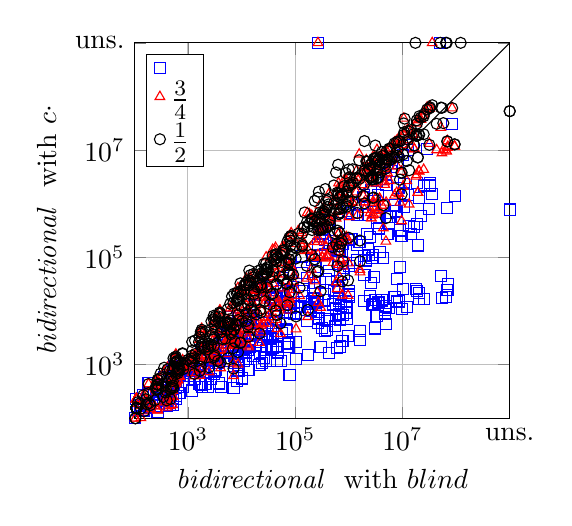
\begin{tikzpicture}[scale=1]
\begin{axis}[grid=major,height=2.5in, legend cell align=right, width=2.5in,xlabel style={align=center}, xlabel={\emph{bidirectional} \bddastar{} with $\heu{blind}{}$}, xmin=100, xmax=1000000001, xmode=log, ylabel style={align=center}, ylabel={\emph{bidirectional} \bddastar{} with $c \cdot \perfecth$}, ymin=100, ymax=1000000001, ymode=log,legend pos=north west,xticklabels={$10^3$, $10^5$, $10^7$, uns.},yticklabels={$10^3$, $10^5$, $10^7$, uns.}]
%legend style={anchor=north east}
\addplot[only marks,mark=square,blue] coordinates {
(45014.000000, 2254.000000) (799.000000, 383.000000) (420828.000000, 1672.000000) (2681.000000, 2093.000000) (5598.000000, 3439.000000) (7953.000000, 2715.000000) (206890.000000, 15639.000000) (775653.000000, 180934.000000) (1154900.000000, 665770.000000) (642523.000000, 134507.000000) (16629270.000000, 364306.000000) (17354.000000, 20367.000000) (135221.000000, 104201.000000) (8426420.000000, 1966300.000000) (9612729.000000, 249383.000000) (12073290.000000, 11799.000000) (6300.000000, 3576.000000) (78985.000000, 9170.000000) (919216.000000, 7002.000000) (272.000000, 130.000000) (28620.000000, 1191.000000) (1951891.000000, 15308.000000) (248822.000000, 8734.000000) (68668.000000, 4551.000000) (38624.000000, 2026.000000) (878674.000000, 15097.000000) (6305.000000, 1735.000000) (63368.000000, 15062.000000) (2389.000000, 1945.000000) (404.000000, 169.000000) (14615.000000, 7277.000000) (1380076.000000, 941199.000000) (54488340.000000, 17766.000000) (35912080.000000, 1500060.000000) (10553160.000000, 862076.000000) (16629270.000000, 364306.000000) (361.000000, 580.000000) (2197100.000000, 268553.000000) (291382.000000, 34633.000000) (184986.000000, 11960.000000) (45447.000000, 3256.000000) (580.000000, 731.000000) (253.000000, 195.000000) (3022730.000000, 1141071.000000) (16994.000000, 10154.000000) (969624.000000, 3458.000000) (20652300.000000, 1284075.000000) (5591.000000, 3429.000000) (66879190.000000, 24947.000000) (659.000000, 766.000000) (270469.000000, 7008.000000) (586.000000, 754.000000) (685332.000000, 47337.000000) (110.000000, 227.000000) (6.000000, 6.000000) (2928250.000000, 938745.000000) (12493220.000000, 1432032.000000) (1195321.000000, 79569.000000) (4908.000000, 3651.000000) (1013261.000000, 24026.000000) (68619943.000000, 845215.000000) (291382.000000, 34633.000000) (12212.000000, 6471.000000) (578727.000000, 11222.000000) (171764.000000, 1510.000000) (45889.000000, 1170.000000) (69400430.000000, 24782.000000) (91575.000000, 28067.000000) (1407139.000000, 88324.000000) (2779849.000000, 111258.000000) (2508080.000000, 19269.000000) (17.000000, 17.000000) (110.000000, 227.000000) (12316.000000, 1726.000000) (110.000000, 227.000000) (2197100.000000, 268553.000000) (110.000000, 227.000000) (110.000000, 227.000000) (271546.000000, 173857.000000) (32516920.000000, 2191907.000000) (6443.000000, 3979.000000) (4092.000000, 1793.000000) (667192.000000, 443080.000000) (3295900.000000, 8184.000000) (1621267.000000, 4294.000000) (717728.000000, 12645.000000) (2948540.000000, 42999.000000) (6134.000000, 3009.000000) (578485.000000, 8178.000000) (685810.000000, 140253.000000) (5465.000000, 1625.000000) (696387.000000, 6977.000000) (16929.000000, 4385.000000) (7839360.000000, 15064.000000) (30320.000000, 2245.000000) (319188.000000, 4897.000000) (68.000000, 126.000000) (239.000000, 167.000000) (6145.000000, 7602.000000) (29106.000000, 1877.000000) (5995101.000000, 576764.000000) (18485830.000000, 2424135.000000) (110.000000, 227.000000) (327.000000, 391.000000) (9538.000000, 2387.000000) (6648.000000, 3100.000000) (3352587.000000, 444227.000000) (8612.000000, 775.000000) (988936.000000, 20322.000000) (19.000000, 19.000000) (394004.000000, 6436.000000) (1174.000000, 1065.000000) (75118.000000, 2482.000000) (2552009.000000, 1776307.000000) (9560.000000, 2593.000000) (667.000000, 688.000000) (2463368.000000, 238259.000000) (478.000000, 367.000000) (434519.000000, 318905.000000) (3190.000000, 720.000000) (7735410.000000, 719510.000000) (645.000000, 689.000000) (4022.000000, 1449.000000) (78568.000000, 649.000000) (3268.000000, 1231.000000) (275.000000, 389.000000) (25427960.000000, 2190570.000000) (7313.000000, 1455.000000) (184.000000, 295.000000) (13126.000000, 8149.000000) (8815.000000, 972.000000) (44793.000000, 18168.000000) (498.000000, 607.000000) (110.000000, 227.000000) (7131380.000000, 17901.000000) (3028.000000, 1431.000000) (266686.000000, 14680.000000) (27452.000000, 4682.000000) (110.000000, 227.000000) (3758076.000000, 124220.000000) (1013261.000000, 24026.000000) (84483800.000000, 30757000.000000) (643.000000, 1086.000000) (51982827.000000, 45593.000000) (110.000000, 227.000000) (4947320.000000, 3495783.000000) (47646.000000, 1690.000000) (3758076.000000, 124220.000000) (272.000000, 130.000000) (10821370.000000, 2344109.000000) (5065170.000000, 560444.000000) (6305.000000, 3688.000000) (795.000000, 692.000000) (7066.000000, 2151.000000) (1812.000000, 1685.000000) (22852.000000, 3232.000000) (1866779.000000, 1325092.000000) (3807.000000, 447.000000) (1932.000000, 1745.000000) (4429.000000, 2997.000000) (1026547.000000, 18173.000000) (3032.000000, 1182.000000) (34735.000000, 17347.000000) (821875.000000, 49176.000000) (2977.000000, 1564.000000) (114169.000000, 11993.000000) (648412.000000, 16649.000000) (526273.000000, 160732.000000) (3065.000000, 761.000000) (1816.000000, 1431.000000) (3425027.000000, 548619.000000) (35379.000000, 2009.000000) (990788.000000, 215307.000000) (514.000000, 438.000000) (3935.000000, 2575.000000) (120989.000000, 12569.000000) (23137.000000, 2270.000000) (2390.000000, 385.000000) (4406200.000000, 97714.000000) (349.000000, 219.000000) (19.000000, 24.000000) (1592435.000000, 191524.000000) (585966.000000, 10825.000000) (3903.000000, 2661.000000) (608088.000000, 36945.000000) (105.000000, 102.000000) (13233.000000, 1901.000000) (665896.000000, 15502.000000) (26188.000000, 6995.000000) (103731.000000, 1276.000000) (5685520.000000, 11218.000000) (4253394.000000, 944675.000000) (24827010.000000, 2118702.000000) (13453.000000, 806.000000) (19360747.000000, 167248.000000) (93855725.000000, 1410874.000000) (288944.000000, 110331.000000) (592.000000, 599.000000) (1772.000000, 1234.000000) (17.000000, 17.000000) (69.000000, 127.000000) (70049400.000000, 32040.000000) (761171.000000, 2729.000000) (167318.000000, 41072.000000) (711.000000, 294.000000) (422.000000, 404.000000) (18598290.000000, 425706.000000) (83627.000000, 13293.000000) (31784030.000000, 796128.000000) (14685750.000000, 276776.000000) (110.000000, 227.000000) (3720.000000, 1080.000000) (5680770.000000, 412791.000000) (11307.000000, 1194.000000) (1754.000000, 1051.000000) (206369.000000, 13391.000000) (206890.000000, 15639.000000) (110.000000, 227.000000) (482.000000, 273.000000) (13503.000000, 6331.000000) (293467.000000, 255620.000000) (982346.000000, 728902.000000) (41064.000000, 9802.000000) (16565.000000, 3956.000000) (110.000000, 227.000000) (20591110.000000, 16692.000000) (450847.000000, 7118.000000) (2777692.000000, 936625.000000) (83627.000000, 13293.000000) (4861336.000000, 2232981.000000) (228384.000000, 32860.000000) (26399.000000, 3331.000000) (1960009.000000, 46813.000000) (835.000000, 862.000000) (1026547.000000, 18173.000000) (35.000000, 35.000000) (357386.000000, 21065.000000) (3083.000000, 673.000000) (1142.000000, 753.000000) (595.000000, 501.000000) (43020.000000, 17113.000000) (3120540.000000, 4738.000000) (146131.000000, 18737.000000) (13310070.000000, 386242.000000) (199726.000000, 10270.000000) (128.000000, 174.000000) (552854.000000, 5334.000000) (523.000000, 353.000000) (110.000000, 227.000000) (5590.000000, 3439.000000) (1313.000000, 862.000000) (365068.000000, 6987.000000) (1741.000000, 1005.000000) (2885.000000, 1841.000000) (110.000000, 227.000000) (504.000000, 376.000000) (9612729.000000, 249383.000000) (2627892.000000, 33210.000000) (41279.000000, 12883.000000) (200.000000, 165.000000) (58954.000000, 41212.000000) (276116.000000, 7385.000000) (4673790.000000, 10545.000000) (235627.000000, 65349.000000) (598.000000, 768.000000) (707.000000, 629.000000) (44793.000000, 18168.000000) (11263.000000, 2763.000000) (15.000000, 20.000000) (20286.000000, 34224.000000) (1000000000, 779118.000000) (110.000000, 227.000000) (653.000000, 387.000000) (64653630.000000, 18428.000000) (78568.000000, 649.000000) (81694.000000, 11766.000000) (6954.000000, 582.000000) (3134.000000, 1253.000000) (24119.000000, 5898.000000) (1119621.000000, 223156.000000) (321573.000000, 282201.000000) (309.000000, 328.000000) (13940.000000, 2376.000000) (16675.000000, 1441.000000) (153.000000, 140.000000) (319188.000000, 4897.000000) (22502.000000, 25216.000000) (24880960.000000, 16809.000000) (778501.000000, 63318.000000) (134838.000000, 51590.000000) (13878.000000, 2214.000000) (39131.000000, 3729.000000) (150391.000000, 14784.000000) (148.000000, 269.000000) (4149270.000000, 15763.000000) (3398176.000000, 2701952.000000) (823.000000, 830.000000) (8557.000000, 7289.000000) (1671.000000, 445.000000) (4979.000000, 2206.000000) (231318.000000, 14096.000000) (1731.000000, 428.000000) (8963770.000000, 65682.000000) (263139.000000, 5912.000000) (654223.000000, 26834.000000) (53737.000000, 23206.000000) (173.000000, 169.000000) (13705.000000, 2125.000000) (275.000000, 389.000000) (20126040.000000, 21710.000000) (898126.000000, 9104.000000) (110.000000, 227.000000) (1648.000000, 768.000000) (1951891.000000, 15308.000000) (3615352.000000, 346156.000000) (1819.000000, 383.000000) (25911.000000, 1323.000000) (447654.000000, 466479.000000) (1449216.000000, 607783.000000) (472.000000, 257.000000) (1610.000000, 436.000000) (610768.000000, 2072.000000) (57378.000000, 3874.000000) (110.000000, 227.000000) (102192.000000, 2628.000000) (110.000000, 227.000000) (37971.000000, 15153.000000) (23291.000000, 4180.000000) (8073.000000, 1385.000000) (7133.000000, 1901.000000) (654223.000000, 26834.000000) (10616870.000000, 1551453.000000) (7248.000000, 4166.000000) (1358.000000, 693.000000) (740544.000000, 176382.000000) (17804760.000000, 25972.000000) (527257.000000, 24138.000000) (8149.000000, 505.000000) (1018.000000, 846.000000) (23163.000000, 26932.000000) (10222840.000000, 25416.000000) (399705.000000, 76614.000000) (2627892.000000, 33210.000000) (33.000000, 33.000000) (12309.000000, 1298.000000) (681267.000000, 2178.000000) (2713041.000000, 12855.000000) (18958.000000, 2904.000000) (14044.000000, 8441.000000) (44901.000000, 2137.000000) (8646680.000000, 15109.000000) (1200.000000, 329.000000) (520.000000, 178.000000) (164623.000000, 6550.000000) (32.000000, 32.000000) (1958336.000000, 107919.000000) (30.000000, 35.000000) (2009325.000000, 609786.000000) (8454.000000, 2133.000000) (3631.000000, 1181.000000) (275.000000, 435.000000) (2686.000000, 1364.000000) (4970407.000000, 12187.000000) (2468.000000, 731.000000) (19.000000, 24.000000) (31.000000, 46.000000) (71690.000000, 9778.000000) (2702.000000, 543.000000) (12843646.000000, 10155900.000000) (547.000000, 924.000000) (7104.000000, 372.000000) (110.000000, 227.000000) (9033600.000000, 318539.000000) (53737.000000, 23206.000000) (23946.000000, 1072.000000) (643.000000, 1086.000000) (64.000000, 105.000000) (458.000000, 761.000000) (5247892.000000, 268649.000000) (6159990.000000, 4106010.000000) (365911.000000, 4234.000000) (26915.000000, 4870.000000) (19360747.000000, 167248.000000) (43593.000000, 4327.000000) (13499.000000, 797.000000) (18480360.000000, 23468.000000) (15437.000000, 2899.000000) (346655.000000, 15762.000000) (19.000000, 19.000000) (272.000000, 130.000000) (105.000000, 102.000000) (650.000000, 426.000000) (110.000000, 227.000000) (416.000000, 527.000000) (3510187.000000, 14231.000000) (93855725.000000, 1410874.000000) (221952.000000, 17450.000000) (4919140.000000, 5730.000000) (1000000000, 779118.000000) (7845.000000, 1985.000000) (41064.000000, 9802.000000) (30176.000000, 4643.000000) (2756053.000000, 98403.000000) (2124.000000, 439.000000) (536.000000, 235.000000) (17644.000000, 3806.000000) (110.000000, 227.000000) (11427.000000, 3974.000000) (3306.000000, 785.000000) (363196.000000, 116331.000000) (16248.000000, 7362.000000) (110.000000, 227.000000) (8573.000000, 1057.000000) (906510.000000, 11687.000000) (9560.000000, 2593.000000) (7108440.000000, 930345.000000) (110.000000, 227.000000) (4677569.000000, 8924.000000) (64.000000, 104.000000) (30894.000000, 3397.000000) (617751.000000, 137260.000000) (297822.000000, 2148.000000) (15937920.000000, 12657580.000000) (632582.000000, 28361.000000) (1229.000000, 886.000000) (5492.000000, 1169.000000) (21617.000000, 990.000000) (19.000000, 24.000000) (8179875.000000, 5858120.000000) (3157240.000000, 15925.000000) (399280.000000, 4384.000000) (20.000000, 20.000000) (1376.000000, 551.000000) (7941450.000000, 40008.000000) (44694.000000, 7885.000000) (9650.000000, 3283.000000) (3892224.000000, 2872860.000000) (110.000000, 227.000000) (53523.000000, 1190.000000) (29639.000000, 3065.000000) (5332.000000, 2360.000000) (133.000000, 95.000000) (2948540.000000, 42999.000000) (1910483.000000, 1429008.000000) (76616.000000, 2170.000000) (146131.000000, 18737.000000) (19553.000000, 25059.000000) (7607.000000, 1081.000000) (1400000.000000, 171126.000000) (185.000000, 450.000000) (611.000000, 260.000000) (684.000000, 297.000000) (5247892.000000, 268649.000000) (37873.000000, 28975.000000) (9574.000000, 4286.000000) (28816170.000000, 10373150.000000) (1798.000000, 1883.000000) (75688.000000, 48420.000000) (402.000000, 224.000000) (2280129.000000, 140909.000000) (2886445.000000, 13455.000000) (28727.000000, 24510.000000) (1329.000000, 610.000000) (164.000000, 154.000000) (110.000000, 227.000000) (4671.000000, 2628.000000) (6383199.000000, 4837170.000000) (3022730.000000, 1141071.000000) (8699.000000, 4610.000000) (19.000000, 24.000000) (272.000000, 283.000000) (379461.000000, 38941.000000) (95610.000000, 8689.000000) (664845.000000, 8901.000000) (50753500.000000, 1000000000) (3532561.000000, 1481526.000000) (595.000000, 233.000000) (203819.000000, 91151.000000) (119.000000, 143.000000) (93.000000, 136.000000) (742525.000000, 129156.000000) (1608458.000000, 2838.000000) (1203.000000, 763.000000) (4077.000000, 386.000000) (71876.000000, 2131.000000) (43.000000, 45.000000) (14627.000000, 2133.000000) (82103.000000, 22811.000000) (382.000000, 210.000000) (22219.000000, 1647.000000) (2746.000000, 1226.000000) (60775.000000, 19375.000000) (277.000000, 223.000000) (2354.000000, 1259.000000) (70968.000000, 4322.000000) (272.000000, 130.000000) (5469.000000, 2354.000000) (5675.000000, 3456.000000) (358135.000000, 207932.000000) (32103140.000000, 2405010.000000) (1117.000000, 959.000000) (1562312.000000, 190557.000000) (3577817.000000, 14751.000000) (110.000000, 227.000000) (84284.000000, 11533.000000) (10122.000000, 4834.000000) (399705.000000, 76614.000000) (189.000000, 187.000000) (780238.000000, 8411.000000) (2398355.000000, 112419.000000) (68619943.000000, 845215.000000) (79197.000000, 71199.000000) (4284.000000, 4633.000000) (50768.000000, 6629.000000) (22092620.000000, 597144.000000) (172146.000000, 12076.000000) (9658120.000000, 11002.000000) (110.000000, 227.000000) (2118264.000000, 87738.000000) (8686.000000, 1627.000000) (110.000000, 227.000000) (266187.000000, 1000000000) (110.000000, 227.000000) (256976.000000, 14609.000000) (232622.000000, 26561.000000) (3164.000000, 1486.000000) (293.000000, 339.000000) (9775.000000, 3149.000000) (62066.000000, 15607.000000) (1001352.000000, 70226.000000) (469.000000, 176.000000) (34135.000000, 3078.000000) (110.000000, 227.000000) (74338.000000, 23188.000000) (1713.000000, 1329.000000) (10326634.000000, 8206360.000000) (2041.000000, 820.000000) (12195.000000, 1661.000000) (55577.000000, 23966.000000) (616284.000000, 177043.000000) (67.000000, 67.000000) (327455.000000, 277225.000000) (68.000000, 113.000000) (539.000000, 413.000000) (392.000000, 224.000000) (136079.000000, 24026.000000) (254.000000, 289.000000) (8885.000000, 777.000000) (10225.000000, 553.000000) (420228.000000, 56105.000000) (103274.000000, 9170.000000) (504275.000000, 13273.000000)
};
\addlegendentry{\large$\perfecth$}

\addplot[only marks,mark=triangle,red] coordinates {
(35912080.000000, 1000000000)
(45014.000000, 81953.000000) (799.000000, 1220.000000) (420828.000000, 204951.000000) (2681.000000, 2242.000000) (5598.000000, 6771.000000) (7953.000000, 3544.000000) (206890.000000, 99526.000000) (547.000000, 924.000000) (775653.000000, 1678336.000000) (1154900.000000, 1085974.000000) (642523.000000, 2425230.000000) (16629270.000000, 10497440.000000) (17354.000000, 24106.000000) (135221.000000, 159095.000000) (8426420.000000, 16464310.000000) (9612729.000000, 3984270.000000) (6300.000000, 3939.000000) (78985.000000, 13917.000000) (919216.000000, 204150.000000) (272.000000, 143.000000) (28620.000000, 15795.000000) (1951891.000000, 1072093.000000) (68668.000000, 14856.000000) (38624.000000, 11080.000000) (878674.000000, 2795530.000000) (6305.000000, 2241.000000) (63368.000000, 142725.000000) (2389.000000, 1936.000000) (404.000000, 160.000000) (14615.000000, 42240.000000) (1380076.000000, 1647778.000000) (54488340.000000, 8831640.000000) (990788.000000, 2159123.000000) (10553160.000000, 39031700.000000) (2390.000000, 1344.000000) (361.000000, 749.000000) (2197100.000000, 4889690.000000) (291382.000000, 569290.000000) (184986.000000, 646221.000000) (45447.000000, 14132.000000) (580.000000, 1301.000000) (253.000000, 410.000000) (3022730.000000, 7440690.000000) (16994.000000, 20411.000000) (20652300.000000, 37996610.000000) (5591.000000, 6595.000000) (66879190.000000, 9506270.000000) (659.000000, 727.000000) (504.000000, 376.000000) (270469.000000, 14368.000000) (586.000000, 1510.000000) (685332.000000, 1928844.000000) (110.000000, 231.000000) (6.000000, 6.000000) (2928250.000000, 1056965.000000) (12493220.000000, 24465660.000000) (1195321.000000, 3143640.000000) (4908.000000, 5795.000000) (1013261.000000, 570631.000000) (68619943.000000, 14809370.000000) (291382.000000, 569290.000000) (12212.000000, 40443.000000) (578727.000000, 538271.000000) (171764.000000, 7837.000000) (45889.000000, 4704.000000) (823.000000, 830.000000) (69400430.000000, 11146300.000000) (53737.000000, 102446.000000) (91575.000000, 35647.000000) (1407139.000000, 4172640.000000) (2779849.000000, 2851603.000000) (2508080.000000, 677688.000000) (17.000000, 17.000000) (110.000000, 231.000000) (12316.000000, 4425.000000) (110.000000, 231.000000) (2197100.000000, 4889690.000000) (110.000000, 231.000000) (110.000000, 231.000000) (271546.000000, 316953.000000) (742525.000000, 1477608.000000) (32516920.000000, 65057300.000000) (6443.000000, 3979.000000) (4092.000000, 1888.000000) (667192.000000, 788669.000000) (57856460.000000, 10170640.000000) (3295900.000000, 662825.000000) (1621267.000000, 53264.000000) (717728.000000, 86745.000000) (2948540.000000, 2424930.000000) (6134.000000, 3190.000000) (578485.000000, 166202.000000) (12073290.000000, 2668727.000000) (685810.000000, 1489691.000000) (231318.000000, 196547.000000) (5465.000000, 2901.000000) (696387.000000, 176526.000000) (16929.000000, 5082.000000) (7839360.000000, 1624483.000000) (18598290.000000, 31792780.000000) (319188.000000, 100563.000000) (68.000000, 128.000000) (239.000000, 168.000000) (6145.000000, 11279.000000) (29106.000000, 48732.000000) (5995101.000000, 10808990.000000) (18485830.000000, 36364800.000000) (110.000000, 231.000000) (327.000000, 380.000000) (9538.000000, 21677.000000) (6648.000000, 12626.000000) (3352587.000000, 10150650.000000) (8612.000000, 1018.000000) (988936.000000, 78193.000000) (19.000000, 19.000000) (394004.000000, 110735.000000) (1174.000000, 1387.000000) (75118.000000, 18701.000000) (2552009.000000, 3071860.000000) (9560.000000, 2564.000000) (667.000000, 642.000000) (2463368.000000, 4780270.000000) (478.000000, 451.000000) (434519.000000, 492575.000000) (969624.000000, 19460.000000) (3190.000000, 1925.000000) (7735410.000000, 14882170.000000) (645.000000, 687.000000) (4022.000000, 10091.000000) (78568.000000, 16587.000000) (3268.000000, 4438.000000) (275.000000, 379.000000) (25427960.000000, 52903000.000000) (7313.000000, 6359.000000) (184.000000, 295.000000) (8815.000000, 3444.000000) (44793.000000, 50330.000000) (498.000000, 574.000000) (110.000000, 231.000000) (7131380.000000, 1435484.000000) (3028.000000, 6739.000000) (266686.000000, 111796.000000) (27452.000000, 17695.000000) (110.000000, 231.000000) (3758076.000000, 1248306.000000) (1013261.000000, 570631.000000) (84483800.000000, 60828000.000000) (643.000000, 1184.000000) (51982827.000000, 26328420.000000) (4947320.000000, 5990900.000000) (47646.000000, 14926.000000) (3758076.000000, 1248306.000000) (272.000000, 143.000000) (10821370.000000, 21992040.000000) (5065170.000000, 9742560.000000) (6305.000000, 3688.000000) (795.000000, 950.000000) (7066.000000, 11471.000000) (1812.000000, 4695.000000) (22852.000000, 4033.000000) (1866779.000000, 1384032.000000) (3807.000000, 1826.000000) (1932.000000, 2005.000000) (4429.000000, 2997.000000) (1026547.000000, 1462394.000000) (3032.000000, 5667.000000) (34735.000000, 96976.000000) (821875.000000, 2772370.000000) (2977.000000, 1588.000000) (114169.000000, 312754.000000) (526273.000000, 1045314.000000) (3065.000000, 1639.000000) (1816.000000, 1498.000000) (3425027.000000, 6785700.000000) (35379.000000, 7743.000000) (514.000000, 442.000000) (3935.000000, 10308.000000) (120989.000000, 19296.000000) (23137.000000, 25288.000000) (16629270.000000, 10497440.000000) (4406200.000000, 353246.000000) (349.000000, 202.000000) (19.000000, 22.000000) (1592435.000000, 3085566.000000) (585966.000000, 34772.000000) (3903.000000, 9503.000000) (608088.000000, 717532.000000) (105.000000, 100.000000) (13233.000000, 3164.000000) (665896.000000, 128192.000000) (26188.000000, 13858.000000) (103731.000000, 4609.000000) (5685520.000000, 2690412.000000) (4253394.000000, 8238600.000000) (24827010.000000, 43722690.000000) (13453.000000, 2300.000000) (19360747.000000, 1618818.000000) (93855725.000000, 11779870.000000) (288944.000000, 947179.000000) (592.000000, 643.000000) (1772.000000, 4486.000000) (17.000000, 17.000000) (69.000000, 139.000000) (70049400.000000, 11710700.000000) (761171.000000, 19758.000000) (167318.000000, 677719.000000) (711.000000, 925.000000) (422.000000, 548.000000) (83627.000000, 67862.000000) (31784030.000000, 13214640.000000) (14685750.000000, 23504820.000000) (110.000000, 231.000000) (3720.000000, 3748.000000) (5680770.000000, 10878060.000000) (11307.000000, 7719.000000) (1754.000000, 4074.000000) (206369.000000, 43379.000000) (206890.000000, 99526.000000) (110.000000, 231.000000) (482.000000, 268.000000) (13503.000000, 38120.000000) (293467.000000, 337216.000000) (982346.000000, 1134692.000000) (41064.000000, 68737.000000) (16565.000000, 47185.000000) (110.000000, 231.000000) (20591110.000000, 4023676.000000) (450847.000000, 131027.000000) (2777692.000000, 1050673.000000) (83627.000000, 67862.000000) (4861336.000000, 4452700.000000) (228384.000000, 451615.000000) (1960009.000000, 779515.000000) (835.000000, 951.000000) (1026547.000000, 1462394.000000) (35.000000, 35.000000) (357386.000000, 645107.000000) (3083.000000, 1158.000000) (1142.000000, 1380.000000) (595.000000, 1265.000000) (43020.000000, 152056.000000) (3120540.000000, 1254923.000000) (146131.000000, 181009.000000) (199726.000000, 60162.000000) (128.000000, 171.000000) (1958336.000000, 4662290.000000) (552854.000000, 157311.000000) (523.000000, 330.000000) (110.000000, 231.000000) (5590.000000, 6772.000000) (1313.000000, 1304.000000) (365068.000000, 382979.000000) (1741.000000, 3541.000000) (2885.000000, 2725.000000) (110.000000, 231.000000) (9612729.000000, 3984270.000000) (2627892.000000, 539373.000000) (41279.000000, 139405.000000) (200.000000, 151.000000) (13126.000000, 10875.000000) (58954.000000, 160486.000000) (276116.000000, 218201.000000) (4673790.000000, 2526480.000000) (235627.000000, 588435.000000) (598.000000, 1558.000000) (707.000000, 601.000000) (44793.000000, 50330.000000) (15.000000, 18.000000) (20286.000000, 45199.000000) (110.000000, 231.000000) (653.000000, 526.000000) (64653630.000000, 9871820.000000) (78568.000000, 16587.000000) (81694.000000, 201346.000000) (6954.000000, 1068.000000) (3134.000000, 1432.000000) (24119.000000, 18045.000000) (1119621.000000, 2469547.000000) (321573.000000, 344817.000000) (309.000000, 392.000000) (13940.000000, 24570.000000) (16675.000000, 19244.000000) (153.000000, 136.000000) (319188.000000, 100563.000000) (22502.000000, 29987.000000) (24880960.000000, 4343658.000000) (778501.000000, 68153.000000) (134838.000000, 286227.000000) (13878.000000, 4357.000000) (39131.000000, 32306.000000) (150391.000000, 132329.000000) (148.000000, 269.000000) (4149270.000000, 927915.000000) (3398176.000000, 4103950.000000) (8557.000000, 27085.000000) (1671.000000, 629.000000) (4979.000000, 2647.000000) (1731.000000, 794.000000) (8963770.000000, 1063952.000000) (263139.000000, 194704.000000) (654223.000000, 284371.000000) (53737.000000, 102446.000000) (110.000000, 231.000000) (173.000000, 172.000000) (13705.000000, 8689.000000) (275.000000, 379.000000) (898126.000000, 238346.000000) (110.000000, 231.000000) (1648.000000, 2941.000000) (1951891.000000, 1072093.000000) (3615352.000000, 6027810.000000) (1819.000000, 845.000000) (25911.000000, 5852.000000) (447654.000000, 497119.000000) (1449216.000000, 614844.000000) (472.000000, 261.000000) (1610.000000, 1346.000000) (610768.000000, 26114.000000) (57378.000000, 48555.000000) (110.000000, 231.000000) (102192.000000, 24934.000000) (110.000000, 231.000000) (37971.000000, 139545.000000) (23291.000000, 5447.000000) (8073.000000, 4714.000000) (7133.000000, 2377.000000) (654223.000000, 284371.000000) (10616870.000000, 19382290.000000) (7248.000000, 4435.000000) (1358.000000, 1317.000000) (740544.000000, 200533.000000) (17804760.000000, 3245698.000000) (527257.000000, 1106933.000000) (8149.000000, 3581.000000) (2009325.000000, 3880324.000000) (1018.000000, 876.000000) (23163.000000, 31000.000000) (110.000000, 231.000000) (10222840.000000, 2090053.000000) (399705.000000, 501547.000000) (2627892.000000, 539373.000000) (33.000000, 33.000000) (12309.000000, 3830.000000) (681267.000000, 94554.000000) (2713041.000000, 608844.000000) (18958.000000, 5796.000000) (14044.000000, 30612.000000) (44901.000000, 17821.000000) (8646680.000000, 1545986.000000) (1200.000000, 703.000000) (520.000000, 178.000000) (19.000000, 22.000000) (32.000000, 32.000000) (30.000000, 30.000000) (8454.000000, 7520.000000) (3631.000000, 1181.000000) (275.000000, 510.000000) (2686.000000, 1876.000000) (4970407.000000, 1059481.000000) (2468.000000, 731.000000) (19.000000, 22.000000) (31.000000, 44.000000) (232622.000000, 36232.000000) (2702.000000, 1837.000000) (12843646.000000, 15492680.000000) (7104.000000, 622.000000) (110.000000, 231.000000) (9033600.000000, 14655440.000000) (23946.000000, 10162.000000) (643.000000, 1184.000000) (64.000000, 124.000000) (458.000000, 761.000000) (5247892.000000, 3752200.000000) (6159990.000000, 6644570.000000) (365911.000000, 96548.000000) (26915.000000, 7493.000000) (19360747.000000, 1618818.000000) (43593.000000, 6941.000000) (13499.000000, 2129.000000) (18480360.000000, 3450776.000000) (15437.000000, 7839.000000) (346655.000000, 329304.000000) (19.000000, 19.000000) (648412.000000, 73430.000000) (272.000000, 143.000000) (105.000000, 100.000000) (650.000000, 509.000000) (1176007.000000, 1056882.000000) (416.000000, 889.000000) (3510187.000000, 744005.000000) (93855725.000000, 11779870.000000) (221952.000000, 108100.000000) (4919140.000000, 199390.000000) (7845.000000, 2543.000000) (41064.000000, 68737.000000) (30176.000000, 5893.000000) (2756053.000000, 5485340.000000) (2124.000000, 2422.000000) (536.000000, 251.000000) (17644.000000, 11392.000000) (110.000000, 231.000000) (11427.000000, 4635.000000) (3306.000000, 6356.000000) (16248.000000, 13692.000000) (110.000000, 231.000000) (8573.000000, 10348.000000) (906510.000000, 239768.000000) (9560.000000, 2564.000000) (7108440.000000, 14025030.000000) (110.000000, 231.000000) (4677569.000000, 2276498.000000) (64.000000, 121.000000) (2948540.000000, 2424930.000000) (617751.000000, 1376191.000000) (297822.000000, 11647.000000) (15937920.000000, 19525260.000000) (632582.000000, 1927795.000000) (1229.000000, 904.000000) (5492.000000, 1600.000000) (21617.000000, 2572.000000) (19.000000, 22.000000) (8179875.000000, 9964620.000000) (3157240.000000, 834555.000000) (399280.000000, 102686.000000) (20.000000, 20.000000) (1376.000000, 1520.000000) (7941450.000000, 5014680.000000) (44694.000000, 12651.000000) (9650.000000, 26729.000000) (110.000000, 231.000000) (53523.000000, 3775.000000) (29639.000000, 21303.000000) (20126040.000000, 4081381.000000) (5332.000000, 2281.000000) (363196.000000, 722805.000000) (133.000000, 102.000000) (30894.000000, 26848.000000) (1910483.000000, 2236980.000000) (76616.000000, 16824.000000) (146131.000000, 181009.000000) (19553.000000, 28106.000000) (7607.000000, 2239.000000) (185.000000, 436.000000) (611.000000, 472.000000) (684.000000, 625.000000) (5247892.000000, 3752200.000000) (37873.000000, 43223.000000) (9574.000000, 22928.000000) (28816170.000000, 62662100.000000) (1798.000000, 1978.000000) (75688.000000, 91553.000000) (402.000000, 207.000000) (2280129.000000, 4105040.000000) (2886445.000000, 628797.000000) (28727.000000, 100996.000000) (1329.000000, 617.000000) (164.000000, 217.000000) (110.000000, 231.000000) (469.000000, 171.000000) (4671.000000, 6794.000000) (6383199.000000, 7617980.000000) (3022730.000000, 7440690.000000) (8699.000000, 5909.000000) (164623.000000, 40626.000000) (272.000000, 513.000000) (379461.000000, 156409.000000) (95610.000000, 46672.000000) (664845.000000, 43817.000000) (3532561.000000, 7176400.000000) (595.000000, 441.000000) (203819.000000, 603255.000000) (119.000000, 187.000000) (93.000000, 133.000000) (1608458.000000, 59208.000000) (1203.000000, 1529.000000) (4077.000000, 868.000000) (71876.000000, 10268.000000) (43.000000, 45.000000) (14627.000000, 16891.000000) (82103.000000, 250422.000000) (30320.000000, 34888.000000) (382.000000, 201.000000) (22219.000000, 4604.000000) (2746.000000, 3828.000000) (60775.000000, 26671.000000) (277.000000, 461.000000) (2354.000000, 1314.000000) (70968.000000, 11563.000000) (272.000000, 143.000000) (5469.000000, 2692.000000) (5675.000000, 6841.000000) (358135.000000, 770099.000000) (32103140.000000, 59769000.000000) (1117.000000, 890.000000) (1562312.000000, 8375820.000000) (3577817.000000, 795172.000000) (110.000000, 231.000000) (84284.000000, 285694.000000) (10122.000000, 8091.000000) (55577.000000, 79067.000000) (399705.000000, 501547.000000) (26399.000000, 24487.000000) (189.000000, 186.000000) (13310070.000000, 978646.000000) (780238.000000, 203395.000000) (2398355.000000, 4430150.000000) (11263.000000, 25292.000000) (68619943.000000, 14809370.000000) (79197.000000, 74470.000000) (4284.000000, 4533.000000) (50768.000000, 11367.000000) (22092620.000000, 37302190.000000) (172146.000000, 140670.000000) (9658120.000000, 477733.000000) (110.000000, 231.000000) (2118264.000000, 6554100.000000) (8686.000000, 19013.000000) (110.000000, 231.000000) (266187.000000, 1000000000) (43441480.000000, 10077310.000000) (110.000000, 231.000000) (256976.000000, 22087.000000) (71690.000000, 78434.000000) (3164.000000, 1486.000000) (293.000000, 552.000000) (9775.000000, 8774.000000) (62066.000000, 154637.000000) (1001352.000000, 3068830.000000) (3892224.000000, 3847660.000000) (34135.000000, 9104.000000) (110.000000, 231.000000) (74338.000000, 28335.000000) (1713.000000, 1329.000000) (1400000.000000, 3060070.000000) (10326634.000000, 12603800.000000) (2041.000000, 1369.000000) (12195.000000, 13056.000000) (616284.000000, 205203.000000) (67.000000, 67.000000) (327455.000000, 357848.000000) (68.000000, 122.000000) (539.000000, 1087.000000) (392.000000, 270.000000) (136079.000000, 203106.000000) (254.000000, 515.000000) (10225.000000, 2734.000000) (420228.000000, 1493696.000000) (103274.000000, 179148.000000) (8885.000000, 5879.000000) (504275.000000, 79880.000000)
};
\addlegendentry{\large$\almostperfecth{\frac{3}{4}}$}

\addplot[only marks,mark=o,draw=black] coordinates {
(66879190.000000, 1000000000) (64653630.000000, 1000000000)
(304910.000000, 323726.000000) (45014.000000, 96310.000000) (420828.000000, 1174300.000000) (2681.000000, 3430.000000) (5598.000000, 5975.000000) (7953.000000, 5595.000000) (206890.000000, 513688.000000) (547.000000, 924.000000) (775653.000000, 1451703.000000) (1154900.000000, 1089889.000000) (642523.000000, 1558165.000000) (16629270.000000, 12203870.000000) (17354.000000, 24230.000000) (135221.000000, 159095.000000) (8426420.000000, 14677380.000000) (9612729.000000, 3799350.000000) (12073290.000000, 6270836.000000) (6300.000000, 6658.000000) (78985.000000, 22366.000000) (919216.000000, 881704.000000) (272.000000, 426.000000) (28620.000000, 50168.000000) (1951891.000000, 4106580.000000) (68668.000000, 33024.000000) (878674.000000, 3717630.000000) (6305.000000, 5206.000000) (63368.000000, 125743.000000) (2389.000000, 2478.000000) (404.000000, 216.000000) (14615.000000, 36156.000000) (1380076.000000, 1660764.000000) (54488340.000000, 61545830.000000) (990788.000000, 2053617.000000) (10553160.000000, 31489600.000000) (2390.000000, 1937.000000) (361.000000, 877.000000) (2197100.000000, 6104020.000000) (291382.000000, 518769.000000) (184986.000000, 425542.000000) (45447.000000, 31940.000000) (580.000000, 1114.000000) (253.000000, 389.000000) (3022730.000000, 7021860.000000) (16994.000000, 20544.000000) (969624.000000, 37377.000000) (20652300.000000, 42821500.000000) (5591.000000, 5948.000000) (659.000000, 822.000000) (504.000000, 376.000000) (270469.000000, 55872.000000) (586.000000, 1283.000000) (685332.000000, 1362276.000000) (110.000000, 155.000000) (6.000000, 6.000000) (2928250.000000, 1305452.000000) (12493220.000000, 22620150.000000) (1195321.000000, 2462907.000000) (4908.000000, 6070.000000) (1013261.000000, 2212912.000000) (68619943.000000, 14562170.000000) (291382.000000, 518769.000000) (12212.000000, 30624.000000) (578727.000000, 3821529.000000) (171764.000000, 10461.000000) (45889.000000, 8371.000000) (53737.000000, 109906.000000) (91575.000000, 47619.000000) (1407139.000000, 3057506.000000) (2779849.000000, 3264669.000000) (2508080.000000, 5307550.000000) (17.000000, 17.000000) (110.000000, 155.000000) (12316.000000, 6491.000000) (110.000000, 155.000000) (2197100.000000, 6104020.000000) (110.000000, 155.000000) (110.000000, 155.000000) (271546.000000, 319833.000000) (32516920.000000, 63058900.000000) (6443.000000, 3979.000000) (4092.000000, 3985.000000) (667192.000000, 795302.000000) (57856460.000000, 31885500.000000) (3295900.000000, 2931439.000000) (1621267.000000, 84983.000000) (717728.000000, 182022.000000) (2948540.000000, 6889380.000000) (6134.000000, 5641.000000) (578485.000000, 782360.000000) (2886445.000000, 2889055.000000) (685810.000000, 1308707.000000) (5465.000000, 10754.000000) (696387.000000, 841841.000000) (16929.000000, 9518.000000) (7839360.000000, 7794970.000000) (30320.000000, 64945.000000) (319188.000000, 665080.000000) (68.000000, 103.000000) (239.000000, 216.000000) (14627.000000, 46690.000000) (6145.000000, 13650.000000) (29106.000000, 60390.000000) (5995101.000000, 10614500.000000) (18485830.000000, 35874610.000000) (110.000000, 155.000000) (327.000000, 402.000000) (9538.000000, 32797.000000) (6648.000000, 18786.000000) (3352587.000000, 7335320.000000) (8612.000000, 1716.000000) (988936.000000, 232851.000000) (19.000000, 19.000000) (394004.000000, 379040.000000) (1174.000000, 1469.000000) (75118.000000, 78768.000000) (2552009.000000, 3094240.000000) (9560.000000, 2564.000000) (667.000000, 769.000000) (2463368.000000, 4378389.000000) (478.000000, 571.000000) (434519.000000, 492575.000000) (3190.000000, 5605.000000) (23137.000000, 59426.000000) (7735410.000000, 14043360.000000) (645.000000, 859.000000) (4022.000000, 9108.000000) (78568.000000, 47861.000000) (22219.000000, 10512.000000) (3268.000000, 7885.000000) (275.000000, 350.000000) (25427960.000000, 46992210.000000) (7313.000000, 21173.000000) (184.000000, 295.000000) (399280.000000, 368801.000000) (38624.000000, 21403.000000) (8815.000000, 8656.000000) (44793.000000, 110789.000000) (498.000000, 574.000000) (7131380.000000, 7407866.000000) (1119621.000000, 2314029.000000) (3028.000000, 7058.000000) (266686.000000, 558898.000000) (27452.000000, 60472.000000) (110.000000, 155.000000) (3758076.000000, 5408040.000000) (1013261.000000, 2212912.000000) (84483800.000000, 60828000.000000) (643.000000, 1184.000000) (4947320.000000, 6031540.000000) (47646.000000, 100428.000000) (3758076.000000, 5408040.000000) (272.000000, 426.000000) (10821370.000000, 21584860.000000) (5065170.000000, 9640030.000000) (6305.000000, 3688.000000) (795.000000, 1632.000000) (7066.000000, 14148.000000) (1812.000000, 4483.000000) (22852.000000, 9475.000000) (1866779.000000, 1385361.000000) (3807.000000, 6276.000000) (1932.000000, 2410.000000) (4429.000000, 2997.000000) (1026547.000000, 3098000.000000) (821875.000000, 2122389.000000) (2977.000000, 2950.000000) (114169.000000, 277741.000000) (648412.000000, 136476.000000) (526273.000000, 1019615.000000) (3065.000000, 2251.000000) (1816.000000, 2137.000000) (3425027.000000, 6188250.000000) (35379.000000, 20494.000000) (35912080.000000, 68684200.000000) (514.000000, 799.000000) (3935.000000, 8894.000000) (120989.000000, 27324.000000) (16629270.000000, 12203870.000000) (4406200.000000, 945065.000000) (349.000000, 250.000000) (19.000000, 22.000000) (1592435.000000, 2928773.000000) (585966.000000, 176089.000000) (3903.000000, 9429.000000) (608088.000000, 1606648.000000) (105.000000, 100.000000) (13233.000000, 4988.000000) (665896.000000, 290193.000000) (26188.000000, 48972.000000) (799.000000, 1589.000000) (103731.000000, 7930.000000) (4253394.000000, 7774220.000000) (24827010.000000, 42593550.000000) (13453.000000, 3332.000000) (93855725.000000, 12802980.000000) (288944.000000, 686042.000000) (592.000000, 672.000000) (1772.000000, 4121.000000) (17.000000, 17.000000) (3577817.000000, 3151953.000000) (761171.000000, 35553.000000) (167318.000000, 464561.000000) (711.000000, 1138.000000) (422.000000, 569.000000) (18598290.000000, 31108180.000000) (83627.000000, 114094.000000) (31784030.000000, 12547900.000000) (14685750.000000, 23787910.000000) (110.000000, 155.000000) (3720.000000, 7929.000000) (5680770.000000, 10694220.000000) (11307.000000, 30819.000000) (1754.000000, 3792.000000) (206369.000000, 323429.000000) (206890.000000, 513688.000000) (110.000000, 155.000000) (482.000000, 374.000000) (13503.000000, 37183.000000) (293467.000000, 338913.000000) (982346.000000, 1134692.000000) (41064.000000, 90297.000000) (16565.000000, 42321.000000) (110.000000, 155.000000) (20591110.000000, 19326550.000000) (450847.000000, 399695.000000) (2777692.000000, 1283426.000000) (83627.000000, 114094.000000) (4861336.000000, 4480120.000000) (228384.000000, 457647.000000) (1449216.000000, 671814.000000) (1960009.000000, 1017496.000000) (835.000000, 962.000000) (1026547.000000, 3098000.000000) (35.000000, 35.000000) (357386.000000, 620007.000000) (3083.000000, 1389.000000) (1142.000000, 1304.000000) (43020.000000, 114216.000000) (3120540.000000, 12175720.000000) (146131.000000, 362275.000000) (13310070.000000, 4214630.000000) (199726.000000, 112157.000000) (128.000000, 191.000000) (552854.000000, 281103.000000) (523.000000, 494.000000) (110.000000, 155.000000) (5590.000000, 5976.000000) (1313.000000, 1317.000000) (365068.000000, 1878362.000000) (2885.000000, 3735.000000) (110.000000, 155.000000) (9612729.000000, 3799350.000000) (2627892.000000, 3111040.000000) (41279.000000, 91669.000000) (200.000000, 176.000000) (13126.000000, 13499.000000) (58954.000000, 136338.000000) (276116.000000, 1681248.000000) (4673790.000000, 5779282.000000) (235627.000000, 477395.000000) (598.000000, 1325.000000) (707.000000, 814.000000) (44793.000000, 110789.000000) (15.000000, 18.000000) (20286.000000, 55587.000000) (1000000000, 53254200.000000) (110.000000, 155.000000) (653.000000, 1019.000000) (110.000000, 155.000000) (78568.000000, 47861.000000) (81694.000000, 166892.000000) (6954.000000, 2014.000000) (3134.000000, 3232.000000) (24119.000000, 44762.000000) (321573.000000, 345765.000000) (309.000000, 679.000000) (13940.000000, 56813.000000) (16675.000000, 49184.000000) (153.000000, 136.000000) (319188.000000, 665080.000000) (22502.000000, 29987.000000) (24880960.000000, 19768890.000000) (778501.000000, 84695.000000) (134838.000000, 278528.000000) (13878.000000, 15778.000000) (39131.000000, 55327.000000) (150391.000000, 687317.000000) (148.000000, 269.000000) (4149270.000000, 9232370.000000) (3398176.000000, 4168510.000000) (823.000000, 830.000000) (8557.000000, 22051.000000) (1671.000000, 766.000000) (4979.000000, 3042.000000) (231318.000000, 1132129.000000) (1731.000000, 918.000000) (8963770.000000, 2815960.000000) (263139.000000, 1291973.000000) (654223.000000, 642418.000000) (53737.000000, 109906.000000) (51982827.000000, 61977320.000000) (110.000000, 155.000000) (173.000000, 182.000000) (13705.000000, 30028.000000) (275.000000, 350.000000) (898126.000000, 959824.000000) (110.000000, 155.000000) (69.000000, 98.000000) (1648.000000, 3282.000000) (1951891.000000, 4106580.000000) (3615352.000000, 6542800.000000) (1819.000000, 1273.000000) (25911.000000, 45344.000000) (447654.000000, 497119.000000) (472.000000, 350.000000) (1610.000000, 2653.000000) (610768.000000, 68536.000000) (57378.000000, 121471.000000) (110.000000, 155.000000) (102192.000000, 94902.000000) (37971.000000, 107774.000000) (23291.000000, 27370.000000) (8073.000000, 15511.000000) (7133.000000, 4423.000000) (654223.000000, 642418.000000) (740544.000000, 208619.000000) (10616870.000000, 19353820.000000) (7248.000000, 4503.000000) (1358.000000, 2826.000000) (17804760.000000, 18523600.000000) (527257.000000, 2195036.000000) (8149.000000, 21415.000000) (2009325.000000, 3741687.000000) (1018.000000, 1239.000000) (23163.000000, 31116.000000) (10222840.000000, 8290797.000000) (399705.000000, 870473.000000) (2627892.000000, 3111040.000000) (33.000000, 33.000000) (12309.000000, 9078.000000) (681267.000000, 684992.000000) (2713041.000000, 2827445.000000) (18958.000000, 8669.000000) (14044.000000, 33044.000000) (1741.000000, 4100.000000) (44901.000000, 84775.000000) (8646680.000000, 7450318.000000) (1200.000000, 1813.000000) (520.000000, 409.000000) (164623.000000, 69718.000000) (32.000000, 32.000000) (1958336.000000, 14756580.000000) (30.000000, 30.000000) (8454.000000, 15554.000000) (3631.000000, 1181.000000) (275.000000, 517.000000) (2686.000000, 2305.000000) (4970407.000000, 6668283.000000) (2468.000000, 888.000000) (19.000000, 22.000000) (31.000000, 44.000000) (232622.000000, 92017.000000) (2702.000000, 4538.000000) (12843646.000000, 15652350.000000) (103274.000000, 150742.000000) (7104.000000, 844.000000) (110.000000, 155.000000) (9033600.000000, 14703890.000000) (23946.000000, 51038.000000) (643.000000, 1184.000000) (64.000000, 100.000000) (3032.000000, 8175.000000) (458.000000, 761.000000) (5247892.000000, 6727930.000000) (6159990.000000, 6681040.000000) (632582.000000, 5334400.000000) (365911.000000, 357771.000000) (26915.000000, 15247.000000) (19360747.000000, 7301960.000000) (43593.000000, 10146.000000) (13499.000000, 5552.000000) (18480360.000000, 18579520.000000) (15437.000000, 11187.000000) (346655.000000, 709783.000000) (121886410.000000, 1000000000) (19.000000, 19.000000) (272.000000, 426.000000) (105.000000, 100.000000) (650.000000, 692.000000) (110.000000, 155.000000) (1176007.000000, 4394016.000000) (416.000000, 819.000000) (3510187.000000, 3062953.000000) (93855725.000000, 12802980.000000) (221952.000000, 366044.000000) (4919140.000000, 540045.000000) (1000000000, 53254200.000000) (7845.000000, 5390.000000) (41064.000000, 90297.000000) (30176.000000, 27500.000000) (2756053.000000, 5988530.000000) (2124.000000, 4112.000000) (536.000000, 369.000000) (17644.000000, 15702.000000) (110.000000, 155.000000) (11427.000000, 11033.000000) (3306.000000, 6474.000000) (363196.000000, 795465.000000) (16248.000000, 34204.000000) (110.000000, 155.000000) (8573.000000, 16882.000000) (906510.000000, 1662352.000000) (9560.000000, 2564.000000) (7108440.000000, 13361620.000000) (110.000000, 155.000000) (4677569.000000, 5111837.000000) (64.000000, 100.000000) (2948540.000000, 6889380.000000) (617751.000000, 1398018.000000) (297822.000000, 23400.000000) (15937920.000000, 19742210.000000) (1229.000000, 1115.000000) (5492.000000, 1312.000000) (21617.000000, 3820.000000) (19.000000, 22.000000) (8179875.000000, 10028710.000000) (3157240.000000, 7042210.000000) (20.000000, 20.000000) (1376.000000, 1585.000000) (44694.000000, 31236.000000) (9650.000000, 23395.000000) (110.000000, 155.000000) (53523.000000, 5879.000000) (29639.000000, 51120.000000) (20126040.000000, 19613810.000000) (5332.000000, 4385.000000) (133.000000, 152.000000) (30894.000000, 58693.000000) (1910483.000000, 2236980.000000) (76616.000000, 51799.000000) (146131.000000, 362275.000000) (19553.000000, 28106.000000) (7607.000000, 2676.000000) (185.000000, 436.000000) (611.000000, 1095.000000) (684.000000, 770.000000) (5247892.000000, 6727930.000000) (37873.000000, 43223.000000) (9574.000000, 23352.000000) (742525.000000, 1485228.000000) (1798.000000, 2347.000000) (75688.000000, 92381.000000) (402.000000, 326.000000) (2280129.000000, 4044736.000000) (28727.000000, 76953.000000) (1329.000000, 675.000000) (164.000000, 227.000000) (110.000000, 155.000000) (83282.000000, 252863.000000) (4671.000000, 5540.000000) (6383199.000000, 7617980.000000) (17468670.000000, 1000000000) (3022730.000000, 7021860.000000) (8699.000000, 6800.000000) (19.000000, 22.000000) (272.000000, 524.000000) (379461.000000, 1134025.000000) (95610.000000, 155824.000000) (664845.000000, 158355.000000) (50753500.000000, 1000000000) (3532561.000000, 6804510.000000) (595.000000, 1075.000000) (203819.000000, 532323.000000) (119.000000, 202.000000) (93.000000, 133.000000) (28816170.000000, 57469710.000000) (1608458.000000, 205965.000000) (1203.000000, 2671.000000) (4077.000000, 1098.000000) (71876.000000, 12790.000000) (43.000000, 45.000000) (82103.000000, 206227.000000) (382.000000, 302.000000) (2746.000000, 6423.000000) (60775.000000, 38649.000000) (277.000000, 429.000000) (2354.000000, 2172.000000) (70968.000000, 31711.000000) (272.000000, 426.000000) (5469.000000, 6235.000000) (34735.000000, 79553.000000) (5675.000000, 6108.000000) (358135.000000, 696849.000000) (32103140.000000, 60431500.000000) (1117.000000, 1153.000000) (1562312.000000, 6468330.000000) (110.000000, 155.000000) (84284.000000, 242138.000000) (10122.000000, 19807.000000) (55577.000000, 82280.000000) (399705.000000, 870473.000000) (26399.000000, 75935.000000) (189.000000, 192.000000) (595.000000, 1419.000000) (780238.000000, 855991.000000) (2398355.000000, 4499883.000000) (11263.000000, 25036.000000) (68619943.000000, 14562170.000000) (79197.000000, 90034.000000) (4284.000000, 5073.000000) (50768.000000, 44232.000000) (22092620.000000, 40491750.000000) (172146.000000, 371098.000000) (5685520.000000, 6511274.000000) (9658120.000000, 1503574.000000) (110.000000, 155.000000) (2118264.000000, 6214040.000000) (110.000000, 155.000000) (8686.000000, 18016.000000) (110.000000, 155.000000) (43441480.000000, 31004870.000000) (110.000000, 155.000000) (256976.000000, 53526.000000) (71690.000000, 196390.000000) (3164.000000, 1486.000000) (293.000000, 554.000000) (9775.000000, 12311.000000) (62066.000000, 136572.000000) (1001352.000000, 4379620.000000) (469.000000, 229.000000) (3892224.000000, 3867150.000000) (34135.000000, 13247.000000) (110.000000, 155.000000) (74338.000000, 55350.000000) (1713.000000, 1329.000000) (1400000.000000, 2966842.000000) (10326634.000000, 12759620.000000) (77311.000000, 231169.000000) (2041.000000, 2108.000000) (12195.000000, 33767.000000) (616284.000000, 315431.000000) (67.000000, 67.000000) (327455.000000, 357848.000000) (68.000000, 93.000000) (10990780.000000, 38590900.000000) (539.000000, 1318.000000) (19360747.000000, 7301960.000000) (392.000000, 458.000000) (136079.000000, 169289.000000) (254.000000, 354.000000) (10225.000000, 6489.000000) (420228.000000, 973813.000000) (8885.000000, 16880.000000) (504275.000000, 153912.000000)
};
\addlegendentry{\large$\almostperfecth{\frac{1}{2}}$}

%%%% Line
\addplot[color=black] coordinates {(0.050000, 0.050000) (1000000000, 1000000000)};
\end{axis}
\end{tikzpicture}

            }
        }
    }\\
    \subfloat[Image Time (seconds)\label{fig:bddastar_data_b}]{
        \centering
        \makebox[1\textwidth][c]{
            \resizebox{0.95\textwidth}{!}{
                \includegraphics{figures/image_time-fwd.pdf}
                \hfill
                \includegraphics{figures/image_time-bid.pdf}
            }
        }
    }\\
    \subfloat[Overall Runtime (seconds)\label{fig:bddastar_data_c}]{
        \centering
        \makebox[1\textwidth][c]{
            \resizebox{0.95\textwidth}{!}{
                \includegraphics{figures/overall_search_time-fwd.pdf}
                \hfill
                \includegraphics{figures/overall_search_time-bid.pdf}
            }
        }
    }
    \vspace{-0.2cm}
    %\input{figures/image_time-bid.tex}
    %\input{figures/overall_search_time-bid.tex}
    \caption[Comparison of BDDA$^\star$ with two different heuristics.]{
        Comparison of BDDA$^\star$ with the blind heuristic and with given (fraction) perfect heuristics \autocite{speck-et-al-icaps2020}.
        With \emph{uns.} we refer to instances that were not solved within the time and memory limits.
    }
    %with the blind heuristic \heu{blind}{} and with a given fraction perfect heuristics ($c \in \{1, \frac{3}{4}, \frac{1}{2}\}$)}
    \label{fig:bddastar_data}
\end{figure}

\section{Empirical Results}
\textcite{speck-et-al-icaps2020} empirically investigated forward and bidirectional \bddastar{} with precomputed fraction perfect heuristics on domains from the optimal track from the International Planning Competitions between 1998 and 2018.
A heuristic $c \cdot h$ is called fraction perfect if it assigns to all states the values of the perfect heuristic multiplied by a constant $0 \leq c \leq 1$, where $0\perfecth = \heu{blind}{}$ and $1\perfecth = \perfecth$ are important extreme cases.
Note that \bddastar{} with blind heuristic $0\perfecth = \heu{blind}{}$ corresponds to symbolic blind search.

\Cref{fig:bddastar_data_a} compares the search effort of \bddastar{} with the blind heuristic and the search effort of \bddastar{} with the fraction perfect heuristics.
While the unrealistic case of the perfect heuristic almost always leads to a reduction in search effort in practice, when we consider more realistic cases, namely the fraction perfect heuristic, we can see that the search effort of \bddastar{} can improve or deteriorate to the same extent.

\Cref{fig:bddastar_data_b} shows the expansion time of \bddastar{}, i.e., the cumulative time required to generate all successors with the image operation.
A correlation is observed between the search effort and the expansion time, which also empirically shows that the introduced notion of search effort is an adequate quantity to measure the performance of \bddastar{}.
This highlights the fundamental problem highlighted by \textcite{speck-et-al-icaps2020}: using a heuristic does not always improve the search performance of \bddastar{}.

Finally, \Cref{fig:bddastar_data_c} shows the total running time of \bddastar{} without the time for computing the corresponding heuristic.
Comparing the expansion time with the total running time, we find that \bddastar{} with fraction perfect heuristics has a higher time increase than \bddastar{} with $\heu{blind}{}$, which is due to the time-consuming partitioning of the state sets by heuristic values \autocite{jensen-et-al-aij2008}.

Overall, these empirical results show that also in practice a heuristic can improve or deteriorate the search effort of \bddastar{} to the same extent.
These empirical results are consistent with the presented theoretical results.
Furthermore, \textcite{speck-et-al-icaps2020} show that it appears to be domain
dependent whether a heuristic helps \bddastar{} as the structure of the reachable search space appears to play a central role.

\section{Discussion}\label{sec:symbolic_search_discussion}
As the results of \textcite{speck-et-al-icaps2020} show, using goal-distance estimators, i.e., heuristics, to prune states in symbolic heuristic search does not always pay off.
Indeed, even the perfect heuristic can exponentially deteriorate the search performance of \bddastar{} and other symbolic \astar{} variants.
Since the search performance of \bddastar{} is not directly related to the number of expanded states, but to the size of the involved BDDs during the search, \textcite{speck-et-al-icaps2020} suggest using heuristic functions that can provide a nice structure of the involved decision diagrams or even give a size guarantee.
One possible candidate are potential heuristics \autocite{pommerening-et-al-aaai2015}, which have recently been shown to be encodable as operator potentials within symbolic heuristic search, resulting in state-of-the-art performance \autocite{fiser-et-al-icaps2021wshsdip}.

The fact that symbolic blind search does not use heuristics and yet can compete with explicit heuristic search in cost-optimal planning \autocite{edelkamp-et-al-aaai2015,torralba-et-al-aij2017,speck-et-al-icaps2020} has the advantage that it is not constrained by the limits of heuristics.
Considering expressive extensions of classical planning, such as conditional effects, axioms, and many more, explicit heuristic search planners rarely support them.
The reason is that it is very challenging to design admissible heuristics that are both informative and fast to compute when considering such extensions.
Symbolic blind search, however, provides a good basis to support these extensions, since it does not rely on heuristics and performs an efficient exhaustive search.
In the next chapters, we will take advantage of this and show how symbolic search can be adapted to support expressive extensions in cost-optimal planning.
